% Options for packages loaded elsewhere
% Options for packages loaded elsewhere
\PassOptionsToPackage{unicode}{hyperref}
\PassOptionsToPackage{hyphens}{url}
\PassOptionsToPackage{dvipsnames,svgnames,x11names}{xcolor}
%
\documentclass[
  number,
  preprint]{elsarticle}
\usepackage{xcolor}
\usepackage[margin=0.75in]{geometry}
\usepackage{amsmath,amssymb}
\setcounter{secnumdepth}{5}
\usepackage{iftex}
\ifPDFTeX
  \usepackage[T1]{fontenc}
  \usepackage[utf8]{inputenc}
  \usepackage{textcomp} % provide euro and other symbols
\else % if luatex or xetex
  \usepackage{unicode-math} % this also loads fontspec
  \defaultfontfeatures{Scale=MatchLowercase}
  \defaultfontfeatures[\rmfamily]{Ligatures=TeX,Scale=1}
\fi
\usepackage{lmodern}
\ifPDFTeX\else
  % xetex/luatex font selection
\fi
% Use upquote if available, for straight quotes in verbatim environments
\IfFileExists{upquote.sty}{\usepackage{upquote}}{}
\IfFileExists{microtype.sty}{% use microtype if available
  \usepackage[]{microtype}
  \UseMicrotypeSet[protrusion]{basicmath} % disable protrusion for tt fonts
}{}
\makeatletter
\@ifundefined{KOMAClassName}{% if non-KOMA class
  \IfFileExists{parskip.sty}{%
    \usepackage{parskip}
  }{% else
    \setlength{\parindent}{0pt}
    \setlength{\parskip}{6pt plus 2pt minus 1pt}}
}{% if KOMA class
  \KOMAoptions{parskip=half}}
\makeatother
% Make \paragraph and \subparagraph free-standing
\makeatletter
\ifx\paragraph\undefined\else
  \let\oldparagraph\paragraph
  \renewcommand{\paragraph}{
    \@ifstar
      \xxxParagraphStar
      \xxxParagraphNoStar
  }
  \newcommand{\xxxParagraphStar}[1]{\oldparagraph*{#1}\mbox{}}
  \newcommand{\xxxParagraphNoStar}[1]{\oldparagraph{#1}\mbox{}}
\fi
\ifx\subparagraph\undefined\else
  \let\oldsubparagraph\subparagraph
  \renewcommand{\subparagraph}{
    \@ifstar
      \xxxSubParagraphStar
      \xxxSubParagraphNoStar
  }
  \newcommand{\xxxSubParagraphStar}[1]{\oldsubparagraph*{#1}\mbox{}}
  \newcommand{\xxxSubParagraphNoStar}[1]{\oldsubparagraph{#1}\mbox{}}
\fi
\makeatother


\usepackage{longtable,booktabs,array}
\newcounter{none} % for unnumbered tables
\usepackage{calc} % for calculating minipage widths
% Correct order of tables after \paragraph or \subparagraph
\usepackage{etoolbox}
\makeatletter
\patchcmd\longtable{\par}{\if@noskipsec\mbox{}\fi\par}{}{}
\makeatother
% Allow footnotes in longtable head/foot
\IfFileExists{footnotehyper.sty}{\usepackage{footnotehyper}}{\usepackage{footnote}}
\makesavenoteenv{longtable}
\usepackage{graphicx}
\makeatletter
\newsavebox\pandoc@box
\newcommand*\pandocbounded[1]{% scales image to fit in text height/width
  \sbox\pandoc@box{#1}%
  \Gscale@div\@tempa{\textheight}{\dimexpr\ht\pandoc@box+\dp\pandoc@box\relax}%
  \Gscale@div\@tempb{\linewidth}{\wd\pandoc@box}%
  \ifdim\@tempb\p@<\@tempa\p@\let\@tempa\@tempb\fi% select the smaller of both
  \ifdim\@tempa\p@<\p@\scalebox{\@tempa}{\usebox\pandoc@box}%
  \else\usebox{\pandoc@box}%
  \fi%
}
% Set default figure placement to htbp
\def\fps@figure{htbp}
\makeatother





\setlength{\emergencystretch}{3em} % prevent overfull lines

\providecommand{\tightlist}{%
  \setlength{\itemsep}{0pt}\setlength{\parskip}{0pt}}



 
\usepackage[]{natbib}
\bibliographystyle{elsarticle-num}


\makeatletter
\@ifpackageloaded{caption}{}{\usepackage{caption}}
\AtBeginDocument{%
\ifdefined\contentsname
  \renewcommand*\contentsname{Table of contents}
\else
  \newcommand\contentsname{Table of contents}
\fi
\ifdefined\listfigurename
  \renewcommand*\listfigurename{List of Figures}
\else
  \newcommand\listfigurename{List of Figures}
\fi
\ifdefined\listtablename
  \renewcommand*\listtablename{List of Tables}
\else
  \newcommand\listtablename{List of Tables}
\fi
\ifdefined\figurename
  \renewcommand*\figurename{Figure}
\else
  \newcommand\figurename{Figure}
\fi
\ifdefined\tablename
  \renewcommand*\tablename{Table}
\else
  \newcommand\tablename{Table}
\fi
}
\@ifpackageloaded{float}{}{\usepackage{float}}
\floatstyle{ruled}
\@ifundefined{c@chapter}{\newfloat{codelisting}{h}{lop}}{\newfloat{codelisting}{h}{lop}[chapter]}
\floatname{codelisting}{Listing}
\newcommand*\listoflistings{\listof{codelisting}{List of Listings}}
\makeatother
\makeatletter
\makeatother
\makeatletter
\@ifpackageloaded{caption}{}{\usepackage{caption}}
\@ifpackageloaded{subcaption}{}{\usepackage{subcaption}}
\makeatother
\journal{Template Journal}
\usepackage{bookmark}
\IfFileExists{xurl.sty}{\usepackage{xurl}}{} % add URL line breaks if available
\urlstyle{same}
\hypersetup{
  pdftitle={Deep Neural Network Pipeline for Trajectory Optimization},
  pdfauthor={Kiran M Aralikatti; Dr.~Devendra P. Ghate},
  pdfkeywords={Trajectory Optimization, Deep Neural
Networks, Physics-Informed Neural Networks, Optimal
Control, State-Costate Equations, Indirect Methods},
  colorlinks=true,
  linkcolor={blue},
  filecolor={Maroon},
  citecolor={Blue},
  urlcolor={Blue},
  pdfcreator={LaTeX via pandoc}}


\setlength{\parindent}{6pt}
\begin{document}

\begin{frontmatter}
\title{Deep Neural Network Pipeline for Trajectory Optimization}
\author[1]{Kiran M Aralikatti%
%
}
 \ead{kiranaralikatti6000@gmail.com} 
\author[1]{Dr.~Devendra P. Ghate%
\corref{cor1}%
}
 \ead{devendra.ghate@iist.ac.in} 

\affiliation[1]{organization={Indian Institute of Space Science and
Technology, Department of Aerospace
Engineering},city={Thiruvananthapuram},country={India},countrysep={,},postcodesep={}}

\cortext[cor1]{Corresponding author}


        
\begin{abstract}
This work presents a deep neural network pipeline for trajectory
optimization, focusing on the comparison and analysis of direct and
indirect methods. Indirect methods based on optimal control theory often
suffer from issues such as chattering and sensitivity to initial costate
guesses. To address these challenges, Physics-Informed Neural Networks
(PINNs) are employed to solve the coupled state-costate equations in a
mesh-free manner. Modified activation functions are introduced to
improve PINN convergence and accuracy. A comparative study of the
low-thrust spacecraft (LTS) trajectory optimization problem is conducted
using classical indirect methods and the proposed PINN-based approach.
Through extensive hyperparameter and optimizer tuning, the PINN-based
method achieves accuracy on the order of 10\^{}-10. Furthermore,
random-walk initialized PINNs are used to generate 100,000 high-accuracy
state-control pairs, demonstrating the potential of the approach for
generating training data and solving optimal control problems.
\end{abstract}





\begin{keyword}
    Trajectory Optimization \sep Deep Neural
Networks \sep Physics-Informed Neural Networks \sep Optimal
Control \sep State-Costate Equations \sep 
    Indirect Methods
\end{keyword}
\end{frontmatter}
    

\section{Introduction}\label{introduction}

\subsection{Trajectory Optimization}\label{trajectory-optimization}

Trajectory optimization is a branch of optimal control that focuses on
finding the best possible trajectory, which is a time-parameterized path
of states and control inputs, for a non-autonomous system to achieve a
desired objective. The problem is formulated as an optimization task,
where a \emph{cost function} (also called a performance index) is
minimized or maximized. This cost function can represent fuel
consumption, time, energy, or any other measurable criterion critical to
system performance.

The decision variables in trajectory optimization include the system's
states (such as position, velocity, or orientation) and control inputs
(such as thrust, torque, or steering angle), which evolve over a defined
time horizon. The system dynamics, governed by ordinary differential
equations (ODEs), form the dynamic constraints, ensuring that the
solution respects the laws of physics. Additionally, path constraints
and boundary conditions restrict states and controls within safe or
feasible bounds, such as actuator limits or desired final states.

The optimization problem is often solved numerically using either direct
methods (for example, collocation or direct shooting), which discretize
the trajectory, or indirect methods, which derive necessary conditions
for optimality through the calculus of variations and solve the
resulting two-point boundary value problem (TPBVP). The optimal control
policy must be generated by satisfying all constraints and conditions
that minimize the objective function.

\subsection{General Trajectory Optimization
Problem}\label{general-trajectory-optimization-problem}

Trajectory optimization problems can take various forms depending on the
system's nature and performance objectives. In this thesis, the focus is
limited to continuous-time, single-phase problems where the system
evolves smoothly without any discontinuities in its dynamics. Although
more complex formulations, such as those involving multiple segments or
hybrid systems with discrete transitions, they are outside the scope of
this work.

A general trajectory optimization objective may comprise two components:
a boundary term, represented by \(J(\cdot)\), which captures conditions
at the initial and final time points, and an integral term, represented
by \(w(\cdot)\), which accumulates cost over the entire trajectory
duration. When both terms are included, the problem is said to be in
Bolza form. If only the integral term is present, it is referred to as
the Lagrange form, while a formulation with only the boundary term is
known as the Mayer form.

The optimization is performed over a finite time interval, with time
\(t \in [t_0, t_f]\), where \(t_0\) and \(t_f\) denote the initial and
final times, respectively. The general objective function in Bolza form
is expressed as:

\begin{equation}\protect\phantomsection\label{eq-bolza}{
\min_{t_0, t_f, \mathbf{x}(t), \mathbf{u}(t)} J(t_0, t_f, \mathbf{x}(t_0), \mathbf{x}(t_f)) + \int_{t_0}^{t_f} w(\tau, \mathbf{x}(\tau), \mathbf{u}(\tau)) \, d\tau.
}\end{equation}

Here, the decision variables include the initial and final times
\(t_0, t_f\), as well as the state trajectory \(\mathbf{x}(t)\) and the
control trajectory \(\mathbf{u}(t)\). To ensure feasibility, various
constraints are imposed on these variables.

System dynamics are defined as

\begin{equation}\protect\phantomsection\label{eq-dynamics}{
\dot{\mathbf{x}}(t) = \mathbf{f}(t, \mathbf{x}(t), \mathbf{u}(t))
}\end{equation}

Path constraints restrict the trajectory within specified bounds:

\begin{equation}\protect\phantomsection\label{eq-path-constraints}{
\mathbf{h}(t, \mathbf{x}(t), \mathbf{u}(t)) \leq 0
}\end{equation}

Boundary constraints enforce conditions at the start and end points:

\begin{equation}\protect\phantomsection\label{eq-boundary-constraints}{
\mathbf{g}(t_0, t_F, \mathbf{x}(t_0), \mathbf{x}(t_f)) \leq 0.
}\end{equation}

State, control, and time bounds ensure the solution lies within feasible
ranges:

\begin{equation}\protect\phantomsection\label{eq-bounds}{
\mathbf{x}_\text{low} \leq \mathbf{x}(t) \leq \mathbf{x}_\text{upp}, \quad 
\mathbf{u}_\text{low} \leq \mathbf{u}(t) \leq \mathbf{u}_\text{upp}, \quad 
t_\text{low} \leq t_0 < t_f \leq t_\text{upp}.
}\end{equation}

Initial and final state bounds specify limits at the boundaries:

\begin{equation}\protect\phantomsection\label{eq-initial-final-bounds}{
\mathbf{x}_{0,\text{low}} \leq \mathbf{x}(t_0) \leq \mathbf{x}_{0,\text{upp}}, \quad 
\mathbf{x}_{f,\text{low}} \leq \mathbf{x}(t_f) \leq \mathbf{x}_{f,\text{upp}}.
}\end{equation}

This formulation is suitable for single-phase, continuous-time problems,
focusing on cases expressed in Lagrange form, where only the integral
term is present in the objective function.

\subsection{Modes of Trajectory
Optimization}\label{modes-of-trajectory-optimization}

Trajectory optimization problems can be addressed in two primary modes:
offline and online. In the offline mode, the trajectory is computed
before the actual operation of the system, under the assumption of
complete knowledge of the system dynamics, environment, and control
model. This mode enables complex and accurate optimization, often with
high computational resources. However, it lacks adaptability and becomes
suboptimal when unexpected changes or uncertainties occur during
operation.

The online mode, in contrast, refers to computing or updating the
trajectory in real time during the system's operation. This is
particularly important in the presence of uncertainties, which may arise
from disturbances in the environment, inaccuracies in the system model,
or unmodeled control behavior. Due to the need for rapid computation,
online algorithms prioritize responsiveness over absolute accuracy.

Since offline and online modes each offer distinct advantages and
limitations, a hybrid approach is often employed. In this mode, an
initial trajectory is generated offline based on nominal conditions and
later refined online using real-time state feedback. This allows for a
balance between computational efficiency and adaptability. Deep Neural
Networks (DNNs) are commonly used in such frameworks due to their
ability to generalize from offline training data and adapt quickly
during online execution.

In real-world scenarios, relying solely on precomputed offline
trajectories without incorporating state feedback can result in degraded
performance under uncertainty. Online trajectory optimization
compensates for these deviations by continuously adjusting control
inputs based on the actual system state. Specifically, it aims to
compute the optimal control given the current state, thereby enhancing
robustness and ensuring the system operates effectively in dynamic
environments. The general structure of such algorithms is illustrated in
Figure~\ref{fig-modes}.

\begin{figure}[H]

\begin{minipage}[t]{0.50\linewidth}

\centering{

\pandocbounded{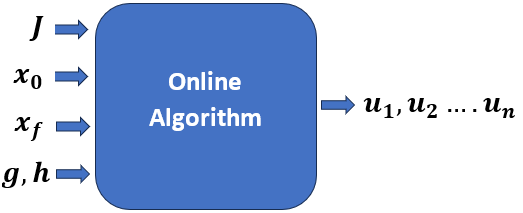
\includegraphics[keepaspectratio]{Chapter1_imgs/offline.PNG}}

}

\subcaption{\label{fig-offline}Offline Optimization}

\end{minipage}%
%
\begin{minipage}[t]{0.50\linewidth}

\centering{

\pandocbounded{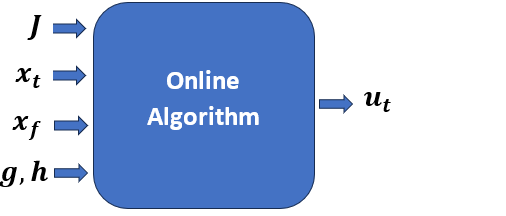
\includegraphics[keepaspectratio]{Chapter1_imgs/online.PNG}}

}

\subcaption{\label{fig-online}Online Optimization}

\end{minipage}%

\caption{\label{fig-modes}Modes of Trajectory Optimization}

\end{figure}%

Looking at aerospace applications, and in particular, retro-propulsive
launch vehicle landing and reaction wheel spacecraft attitude control,
the uncertainties are unavoidable because of the complexity of the
underlying systems and the diversity of the environments under which
these systems operate.

\subsubsection{Algorithms}\label{algorithms}

Keeping in mind the diverse applications of trajectory optimization, and
the conflicting requirements of accuracy and speed, a variety of
algorithms have been developed to solve the trajectory optimization
problem. These algorithms can be broadly classified into two categories:
direct and indirect methods.

In trajectory optimization, direct methods are commonly used to convert
continuous-time problems into nonlinear programming problems. Approaches
like shooting methods, Hermite-Simpson collocation, and pseudospectral
methods differ in how they handle dynamics and discretization. While
shooting methods can struggle with stability over long horizons,
collocation and pseudospectral methods offer improved robustness.

However, the indirect method requires solving a TPBVPs for both the
state and costate ODEs, which poses significant challenges due to the
need for precise boundary conditions. This limitation highlights the
potential of DNNs, which offer a robust alternative by directly solving
these ODEs even with partial or incomplete boundary information, thereby
simplifying the process and expanding the envelope of solvable problems
at the expense of higher computing.

\subsection{Deep Neural Networks}\label{deep-neural-networks}

Machine Learning (ML) is a subset of artificial intelligence that
focuses on enabling systems to learn and adapt from data without
explicit programming. By leveraging algorithms to identify patterns and
optimize representations of input data within a defined space, ML
provides solutions to complex problems across various domains. The
process is guided by feedback signals, enabling systems to refine their
performance iteratively. This methodology has been successfully applied
to challenging tasks such as speech recognition, autonomous navigation,
and predictive modeling, demonstrating its ability to address
specialized, data-driven challenges in diverse fields. A conceptual
relationship among artificial intelligence, machine learning, and deep
learning is illustrated in Figure~\ref{fig-ai-ml-dl}.

The definition given by Prof.~Tom Mitchell is: ``A computer program is
said to learn from experience \(E\) with respect to some task \(T\) and
some performance measure \(P\), if its performance on \(T\), as measured
by \(P\), improves with experience \(E\)'' \citep{chollet2021deep}.

\begin{figure}[H]

\centering{

\centering{

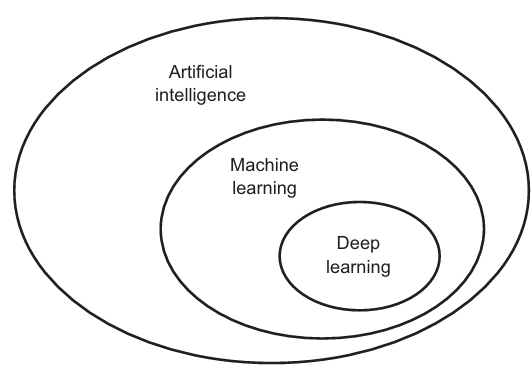
\includegraphics[width=0.6\linewidth,height=\textheight,keepaspectratio]{Chapter1_imgs/c1.PNG}

}

\subcaption{\label{fig-ai-ml-dl}Offline Optimization}

}

\caption{\label{fig-ai-ml-dl}Artificial intelligence, machine learning,
and deep learning \citep{chollet2021deep}}

\end{figure}%

Deep learning is a specialized subfield of machine learning that focuses
on learning hierarchical layers of representations from data. Unlike
traditional machine learning approaches, which typically learn one or
two layers of representations, deep learning involves multiple layers
that progressively capture more meaningful features. These layers are
learned automatically from training data, and the depth of the model
refers to the number of layers. Modern deep learning models, often
implemented using neural networks, can have tens or even hundreds of
layers. Despite the term ``neural network'' being inspired by
neurobiology, deep learning models are not directly related to the
brain's structure or learning mechanisms. Instead, they serve as
mathematical frameworks for learning complex representations from data.
A typical architecture of a DNN is shown in
Figure~\ref{fig-dnn-architecture}, illustrating how layers of neurons
are stacked to form the model.

\begin{figure}[H]

\centering{

\centering{

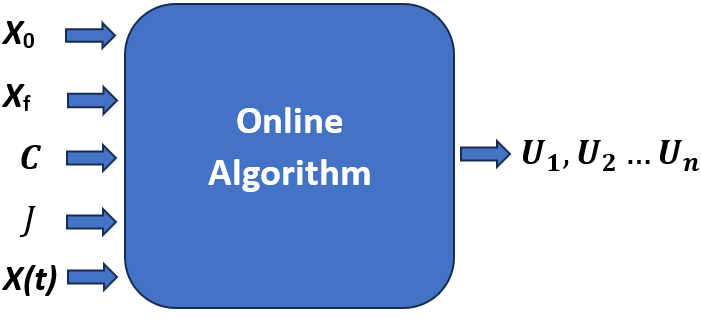
\includegraphics[width=0.6\linewidth,height=\textheight,keepaspectratio]{Chapter1_imgs/c2.PNG}

}

\subcaption{\label{fig-dnn-architecture}Offline Optimization}

}

\caption{\label{fig-dnn-architecture}A typical Deep Neural Network (DNN)
architecture showing multiple layers of neurons \citep{dnn2023}}

\end{figure}%

Since this thesis spans the complete development and application of
various trajectory optimization techniques, ranging from classical
numerical methods to modern deep learning approaches, literature reviews
are integrated contextually at the beginning of each relevant chapter.
For instance, Chapter 2 reviews traditional direct and indirect methods
used in trajectory optimization, while Chapter 3 explores recent
advances in Physics-Informed Neural Networks (PINNs) for solving optimal
control problems. Chapter 4 introduces the Theory of Functional
Connections (TFC), preceded by a review of boundary value
problem-solving methods. Each of these reviews is presented just before
the core technical content to ensure clarity and relevance.

The following section outlines the structure of the thesis and
summarizes the contributions made in each chapter. This overview is
intended to guide the reader through the logical flow of the work and
emphasize the novel aspects of the research.

\subsubsection*{Outline of the Thesis}\label{outline-of-the-thesis}
\addcontentsline{toc}{subsubsection}{Outline of the Thesis}

Chapter 2 presents a comprehensive review of both direct and indirect
methods for solving trajectory optimization problems. It begins with
discretization techniques such as the trapezoidal and Hermite--Simpson
methods, which are applied to the Linear Tangent Steering (LTS) problem.
The chapter also examines the use of regularization strategies to
suppress chattering in control signals. Limitations of direct methods
are discussed, followed by a theoretical introduction to indirect
approaches based on the Pontryagin Maximum Principle.

Chapter 3 focuses on the application of Physics-Informed Neural Networks
(PINNs) for solving optimal control problems. It details the structure
and training of PINNs, emphasizing their capability to simultaneously
learn both state and costate trajectories. The performance of various
activation functions, particularly the Rowdy Adaptive Activation
Function (RAAF), is assessed. Additionally, techniques such as weight
initialization and interpolation are explored to improve training
stability and convergence.

Chapter 4 introduces the Theory of Functional Connections (TFC) as a
powerful method for solving boundary value problems in trajectory
optimization. The mathematical foundations of TFC are presented, and its
application to problems such as energy-optimal planetary landing is
demonstrated. The chapter highlights TFC's ability to analytically
satisfy boundary conditions and handle state and control constraints
with high accuracy.

Finally, Chapter 5 summarizes the key contributions of the thesis and
compares classical numerical methods with learning-based approaches for
trajectory optimization. The strengths and limitations of each method
are discussed, along with potential directions for future work,
including real-time implementation, adaptive control strategies, and
hybrid frameworks that integrate physics-based models with data-driven
techniques.

\newpage

\section{General Methods to Solve Trajectory Optimization
Problem}\label{general-methods-to-solve-trajectory-optimization-problem}

Trajectory optimization problems are typically solved using two broad
families of numerical approaches: discretization-based \emph{direct
transcription} methods, which approximate the optimal control problem by
a finite-dimensional nonlinear program, and \emph{indirect} methods,
which reformulate the problem via the Pontryagin Maximum Principle (PMP)
into a two-point boundary value problem (TPBVP) that must be solved
numerically. This chapter reviews both families and applies them to a
classical benchmark problem in order to expose their respective
strengths and limitations. The motivation for this review is twofold.
First, it establishes the classical optimization background against
which the Physics-Informed Neural Network (PINN) approaches of Chapter 3
are later compared. Second, it makes explicit the TPBVP and
state--costate formulation that PINNs are used to solve in later
chapters.

\subsection{Discretization-Based Direct
Transcription}\label{discretization-based-direct-transcription}

Direct methods for solving optimal control problems (OCPs) involve
transcribing the continuous-time problem into a finite-dimensional
nonlinear programming problem (NLP). This is achieved by discretizing
the time horizon and approximating both the system dynamics and the cost
functional at discrete time points.

Several transcription techniques are used in direct methods, each
differing in the way they discretize the dynamics and integrate the
cost. This thesis considers two widely used collocation-based
techniques: the Trapezoidal method and the Hermite--Simpson method. The
Trapezoidal method is a second-order accurate scheme known for its
simplicity, while the Hermite--Simpson method offers higher
(third-order) accuracy by incorporating midpoint information through
Hermite interpolation and Simpson's integration rule.

The following subsections describe these methods in detail.

\subsubsection{Trapezoidal Method}\label{trapezoidal-method}

The trapezoidal method is a collocation-based discretization scheme that
approximates the dynamics of the system using a second-order accurate
rule. It converts the continuous-time OCPs into an NLP by enforcing
dynamic constraints at discrete time intervals.

As introduced in Chapter 1, we consider a OCP with a Lagrange-type cost
functional:

\begin{equation}\protect\phantomsection\label{eq-ch2-continuous-cost}{
\min_{\mathbf{x}(t), \mathbf{u}(t)} \int_{t_0}^{t_f} w(\mathbf{x}(t), \mathbf{u}(t), t) \, dt,
}\end{equation}

To solve this problem using direct transcription, we apply the
trapezoidal method to discretize both the objective and the dynamics
over a uniform time grid. The time interval \([t_0, t_f]\) is divided
into \(N\) segments, with grid points \(t_0, t_1, \ldots, t_N\), where
\(\Delta t = \frac{t_f - t_0}{N}\) and \(t_k = t_0 + k \Delta t\).

The integral cost functional is approximated as:

\begin{equation}\protect\phantomsection\label{eq-ch2-discrete-cost}{
\min_{\{\mathbf{x}_k, \mathbf{u}_k\}} \sum_{k=0}^{N-1} w(\mathbf{x}_k, \mathbf{u}_k, t_k) \Delta t.
}\end{equation}

The system dynamics are enforced using the trapezoidal rule, resulting
in the collocation constraint:

\begin{equation}\protect\phantomsection\label{eq-ch2-dyn-constraint}{
\mathbf{x}_{k+1} - \mathbf{x}_k - \frac{\Delta t}{2} \left[ \mathbf{f}(\mathbf{x}_k, \mathbf{u}_k, t_k) + \mathbf{f}(\mathbf{x}_{k+1}, \mathbf{u}_{k+1}, t_{k+1}) \right] = 0
}\end{equation}

This discretized optimization problem is also subject to the following
constraints:

\begin{equation}\protect\phantomsection\label{eq-ch2-boundary-conditions}{
\mathbf{x}_0 = \mathbf{x}(t_0), \quad \mathbf{x}_N = \mathbf{x}(t_f)
}\end{equation}

\begin{equation}\protect\phantomsection\label{eq-ch2-path-constraints}{
\mathbf{h}(\mathbf{x}_k, \mathbf{u}_k, t_k) \leq \mathbf{0}, \quad \text{for } k = 0, \dots, N-1
}\end{equation}

\begin{equation}\protect\phantomsection\label{eq-ch2-bounds}{
\mathbf{u}_{\min} \leq \mathbf{u}_k \leq \mathbf{u}_{\max}, \quad \mathbf{x}_{\min} \leq \mathbf{x}_k \leq \mathbf{x}_{\max}
}\end{equation}

The result is a finite-dimensional NLP that can be efficiently solved
using standard numerical optimization techniques, where the decision
variables are the discretized state and control trajectories
\(\{ \mathbf{x}_k, \mathbf{u}_k \}\).

\subsubsection{Hermite--Simpson Method}\label{hermitesimpson-method}

The Hermite--Simpson (H-S) method is a third-order accurate direct
collocation scheme used for solving OCPs. It combines Hermite
interpolation and Simpson's rule to discretize both the dynamics and the
cost functional over a uniform time grid, allowing better approximation
of the system behavior between nodes.

We consider a continuous-time OCP with a Lagrange-type cost functional:

\begin{equation}\protect\phantomsection\label{eq-ch2-hs-cont-cost}{
\min_{\mathbf{x}(t), \mathbf{u}(t)} \int_{t_0}^{t_f} w(\mathbf{x}(t), \mathbf{u}(t), t) \, dt,
}\end{equation}

The time interval \([t_0, t_f]\) is divided into \(N\) uniform segments
with grid points \(t_0, t_1, \ldots, t_N\), and step size
\(\Delta t = \frac{t_f - t_0}{N}\). Midpoints are defined as
\(t_m = \frac{t_k + t_{k+1}}{2}\).

Using Simpson's rule, the discretized cost functional becomes:

\begin{equation}\protect\phantomsection\label{eq-ch2-hs-disc-cost}{
\min_{\{\mathbf{x}_k, \mathbf{u}_k\}} \sum_{k=0}^{N-1} \frac{\Delta t}{6} \left[ w(\mathbf{x}_k, \mathbf{u}_k, t_k) + 4 w(\mathbf{x}_m, \mathbf{u}_m, t_m) + w(\mathbf{x}_{k+1}, \mathbf{u}_{k+1}, t_{k+1}) \right]
}\end{equation}

where \(\mathbf{x}_m\) and \(\mathbf{u}_m\) are midpoint estimates
between \(t_k\) and \(t_{k+1}\).

The system dynamics are enforced using the H-S collocation constraint:

\begin{equation}\protect\phantomsection\label{eq-ch2-hs-dynamics}{
\mathbf{x}_{k+1} = \mathbf{x}_k + \frac{\Delta t}{6} \left[ \mathbf{f}(\mathbf{x}_k, \mathbf{u}_k) + 4 \mathbf{f}(\mathbf{x}_m, \mathbf{u}_m) + \mathbf{f}(\mathbf{x}_{k+1}, \mathbf{u}_{k+1}) \right]
}\end{equation}

The midpoint state \(\mathbf{x}_m\) is approximated as:

\begin{equation}\protect\phantomsection\label{eq-ch2-hs-xm}{
\mathbf{x}_m = \frac{1}{2}(\mathbf{x}_k + \mathbf{x}_{k+1}) + \frac{\Delta t}{8} \left[ \mathbf{f}(\mathbf{x}_k, \mathbf{u}_k) - \mathbf{f}(\mathbf{x}_{k+1}, \mathbf{u}_{k+1}) \right]
}\end{equation}

The full H-S transcription includes the following constraints:

\begin{equation}\protect\phantomsection\label{eq-ch2-hs-bc}{
\mathbf{x}_0 = \mathbf{x}(t_0), \quad \mathbf{x}_N = \mathbf{x}(t_f)
}\end{equation}

\begin{equation}\protect\phantomsection\label{eq-ch2-hs-path}{
\mathbf{h}(\mathbf{x}_k, \mathbf{u}_k) \leq \mathbf{0}, \quad \text{for } k = 0, \dots, N
}\end{equation}

\begin{equation}\protect\phantomsection\label{eq-ch2-hs-bounds}{
\mathbf{u}_{\min} \leq \mathbf{u}_k \leq \mathbf{u}_{\max}, \quad \mathbf{x}_{\min} \leq \mathbf{x}_k \leq \mathbf{x}_{\max}
}\end{equation}

The H-S method achieves higher-order accuracy compared to lower-order
schemes like the trapezoidal method by incorporating interpolated
midpoints in both the cost and dynamic constraints. This enhanced
accuracy makes it especially effective in problems with nonlinear or
rapidly varying dynamics.

\subsection{Linear Tangent Steering Problem}\label{sec-ch2-lts}

The Linear Tangent Steering (LTS) problem \citep{bryson2018applied} is a
classical optimal control problem that involves steering a system
governed by nonlinear dynamics to a specified final state while
minimizing the total control time. It serves as a standard benchmark for
testing the performance of numerical optimization techniques throughout
this thesis.

The objective is to minimize the total time \(t_f\) required to reach a
desired final position from a given initial condition:

\begin{equation}\protect\phantomsection\label{eq-ch2-lts-obj}{
J = \int_0^{t_f} 1 \, dt = t_f
}\end{equation}

\textbf{Dynamic Constraints.} The system is defined by four states:
\(x_1\) and \(x_2\) (position components), and \(x_3\), \(x_4\)
(velocity components). The dynamics are governed by the following
equations:

\begin{equation}\protect\phantomsection\label{eq-ch2-lts-dynamics}{
\begin{aligned}
    \dot{x}_1 &= x_3, \\
    \dot{x}_2 &= x_4, \\
    \dot{x}_3 &= a \cos u, \\
    \dot{x}_4 &= a \sin u,
\end{aligned}
}\end{equation}

where \(a\) is a constant acceleration magnitude, and \(u(t)\) is the
control input representing the steering angle.

\textbf{Boundary Conditions.} The problem is subject to the following
initial and terminal boundary conditions:

\begin{equation}\protect\phantomsection\label{eq-ch2-lts-bc}{
\begin{aligned}
    x_1(0) &= 0, &\quad x_1(t_f) &= \text{free}, \\
    x_2(0) &= 0, &\quad x_2(t_f) &= 5, \\
    x_3(0) &= 0, &\quad x_3(t_f) &= 45, \\
    x_4(0) &= 0, &\quad x_4(t_f) &= 0.
\end{aligned}
}\end{equation}

The analytical solution to this problem is obtained by solving the
necessary conditions of optimality, derived using the Pontryagin Maximum
Principle (PMP). These conditions include the state and costate dynamics
as well as transversality conditions and yield an exact trajectory that
satisfies all constraints.

Figure~\ref{fig-ch2-lts-solution} shows the analytical solution for the
state variables and control input over the optimal trajectory. The
optimized final time is found to be \(t_f = 0.5546 \, \text{s}\), which
serves as a benchmark for evaluating numerical methods.

\begin{figure}

\begin{minipage}[t]{0.50\linewidth}

\centering{

\pandocbounded{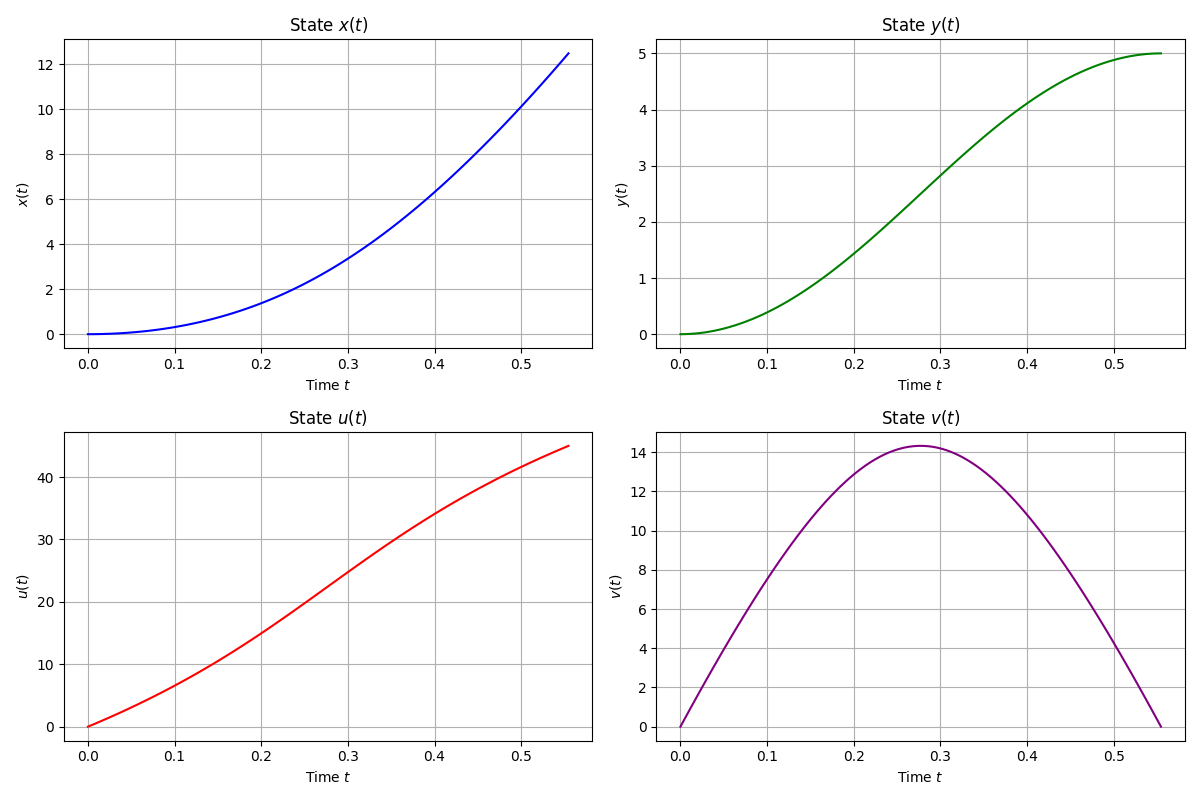
\includegraphics[keepaspectratio]{Chapter2_imgs/c4.png}}

}

\subcaption{\label{fig-ch2-lts-states}State variables
\(x_1, x_2, x_3, x_4\)}

\end{minipage}%
%
\begin{minipage}[t]{0.50\linewidth}

\centering{

\pandocbounded{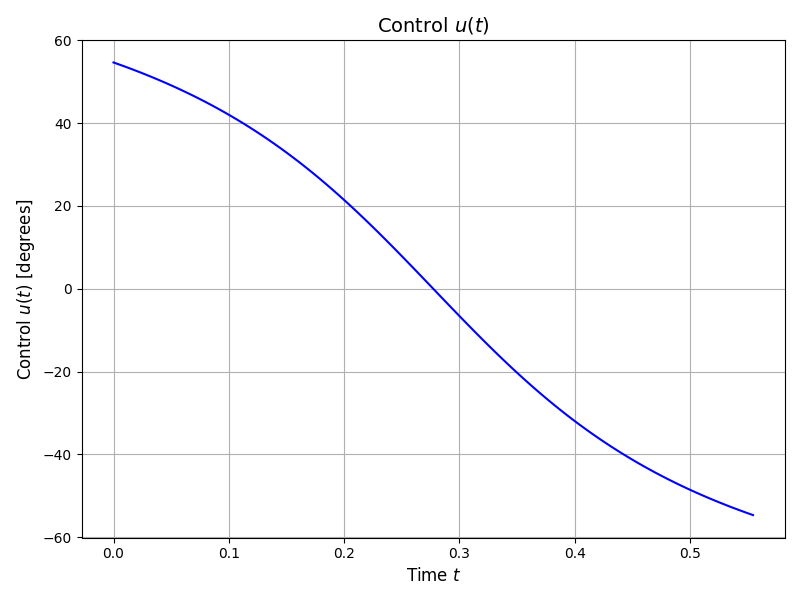
\includegraphics[keepaspectratio]{Chapter2_imgs/c3.png}}

}

\subcaption{\label{fig-ch2-lts-control}Control input \(u(t)\)}

\end{minipage}%

\caption{\label{fig-ch2-lts-solution}Analytical solution}

\end{figure}%

This analytical solution, derived without numerical approximations,
provides a valuable reference for assessing the accuracy and convergence
of transcription-based methods such as the Hermite--Simpson method. For
detailed derivations and analytical formulations, refer to
\citep{bryson2018applied}.

While the analytical solution offers exact results for this benchmark
problem, it is not always feasible for more complex systems or
constraints. Therefore, numerical optimization approaches are employed
to approximate the optimal trajectory using the two direct transcription
techniques introduced earlier, which can be generalized to a broader
class of problems.

\subsubsection{Numerical Optimization
Setup}\label{numerical-optimization-setup}

To numerically solve the LTS problem, the continuous-time optimal
control problem is transcribed into a finite-dimensional NLP problem
using direct collocation methods. The resulting NLP is solved using the
Sequential Least Squares Quadratic Programming (SLSQP) algorithm,
implemented via the \texttt{scipy.optimize.minimize} function in Python.

The optimization procedure minimizes the cost functional while ensuring
that the discretized dynamics, boundary conditions, and path constraints
are satisfied at all collocation points. The discretized design
variables of state vectors, control inputs, and the final time \(t_f\)
across \(N+1\) nodes is given below:

\begin{equation}\protect\phantomsection\label{eq-ch2-design-variables}{
\left[ \tilde{\mathbf{x}}_1,\, \tilde{\mathbf{x}}_2,\, \tilde{\mathbf{x}}_3,\, \tilde{\mathbf{x}}_4,\, \tilde{\mathbf{u}},\, t_f \right]
}\end{equation}

Here \(\tilde{\mathbf{x}}_1\) represents the discretized
\(\mathbf{x_1}\), and the same applies for the other variables.

\textbf{Initial Guess:} A well-chosen initial guess is essential to
ensure the convergence of gradient-based optimization algorithms,
particularly in problems involving nonlinear dynamics and constraints.
The initial guess vector is constructed by concatenating the discretized
design variables are given as below:

\begin{equation}\protect\phantomsection\label{eq-ch2-initial-guess}{
\text{Initial Guess} =
\begin{cases}
\text{Linearly interpolated over the interval } [0, 5] & \text{for } \tilde{\mathbf{x}}_1,\, \tilde{\mathbf{x}}_2, \\
\text{Linearly spaced from } 0 \text{ to } 45 & \text{for } \tilde{\mathbf{x}}_3, \\
0 & \text{for } \tilde{\mathbf{x}}_4, \\
\text{Linearly spaced from } -1 \text{ to } 1 & \text{for } \tilde{\mathbf{u}}, \\
1.0 & \text{for } t_f.
\end{cases}
}\end{equation}

\textbf{Bounds:} To ensure that the optimization remains within feasible
and physically meaningful limits, bounds are imposed on the decision
variables:

\begin{equation}\protect\phantomsection\label{eq-ch2-bounds-setup}{
\text{bounds} =
\begin{cases}
[0, \infty) & \text{for } \tilde{\mathbf{x}}_1, \tilde{\mathbf{x}}_2, \tilde{\mathbf{x}}_3, t_f, \\
(-\infty, \infty) & \text{for } \mathbf{\tilde{x}}_4, \\
[-1.1, 1.1] & \text{for } \mathbf{\tilde{u}}.
\end{cases}
}\end{equation}

These bounds ensure, for example, that horizontal positions and
velocities remain non-negative, while vertical velocities are
unrestricted. The control inputs are slightly relaxed beyond the actual
bounds \([-1, 1]\) to improve solver robustness and prevent premature
clipping due to numerical rounding.

\textbf{Solver Settings:} The optimization solver is configured with
specific parameters to ensure robust and accurate convergence. The
\texttt{SLSQP} (Sequential Least Squares Quadratic Programming)
algorithm is employed as the optimization method. A high maximum
iteration limit is set via \texttt{maxiter=10000}, providing ample
opportunity for convergence. The gradient tolerance is configured with
\texttt{gtol=1e-10}, ensuring that the solution satisfies the
first-order optimality condition with high precision. Additionally,
\texttt{disp=True} enables real-time display of the solver's progress
and convergence messages. These settings collectively help balance
computational cost and accuracy, which is crucial for problems involving
sensitive dynamic constraints and tight boundary conditions.

\subsubsection{Solution using the Trapezoidal
Method}\label{solution-using-the-trapezoidal-method}

Following the numerical setup, the transcribed NLP is solved using the
trapezoidal collocation method. The solver returns the optimal control
\(\tilde{\mathbf{u}}\), the corresponding state trajectories
\(\tilde{\mathbf{x}}_1, \tilde{\mathbf{x}}_2, \tilde{\mathbf{x}}_3, \tilde{\mathbf{x}}_4\),
and the optimal final time \(t_f\).

The results obtained are compared against the analytical solution to
evaluate the performance of the trapezoidal method.
Figure~\ref{fig-ch2-trap-solution} shows the control and state
trajectories computed using the trapezoidal method.

The optimal control law in the LTS problem has a smooth bang-bang
structure, featuring smooth transitions between maximum and minimum
control values. However, the trapezoidal method fails to accurately
capture these transitions, leading to artificial oscillations known as
chattering. This effect is clearly visible in
Figure~\ref{fig-ch2-trap-control}, where the control input fluctuates
excessively around the expected switching points.

\begin{figure}

\begin{minipage}[t]{0.50\linewidth}

\centering{

\pandocbounded{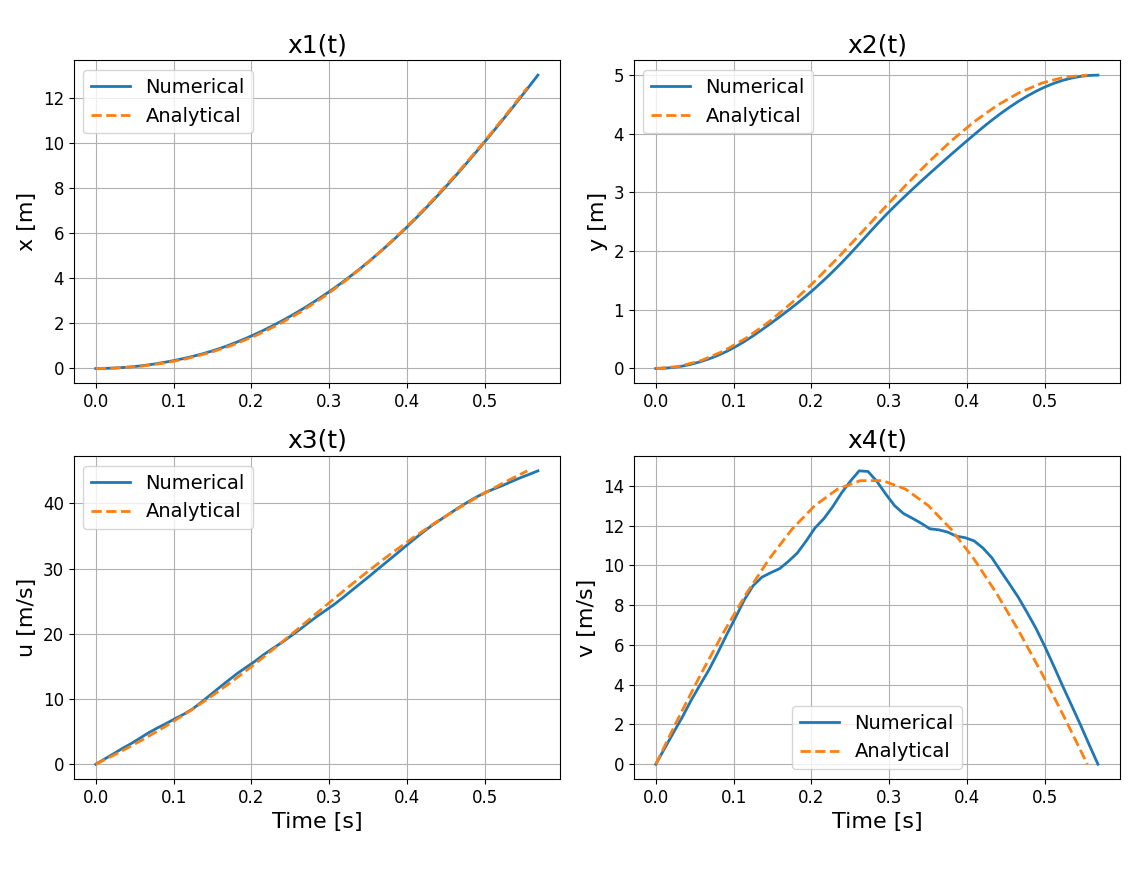
\includegraphics[keepaspectratio]{Chapter2_imgs/trap_state.png}}

}

\subcaption{\label{fig-ch2-trap-state}State variables
\(\tilde{\mathbf{x}}_1, \tilde{\mathbf{x}}_2, \tilde{\mathbf{x}}_3, \tilde{\mathbf{x}}_4\)}

\end{minipage}%
%
\begin{minipage}[t]{0.50\linewidth}

\centering{

\pandocbounded{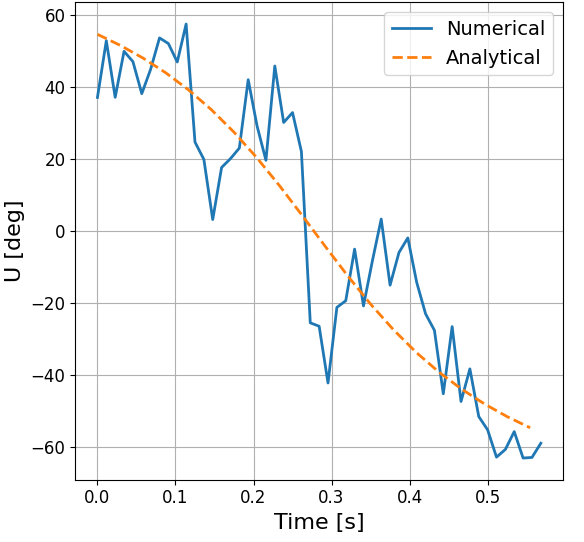
\includegraphics[keepaspectratio]{Chapter2_imgs/trap_control.png}}

}

\subcaption{\label{fig-ch2-trap-control}Control input
\(\mathbf{\tilde{u}}\)}

\end{minipage}%

\caption{\label{fig-ch2-trap-solution}Numerical solution of the LTS
problem using the trapezoidal method.}

\end{figure}%

To quantify the numerical error, the Mean Squared Error (MSE) between
the trapezoidal and analytical solutions is computed for each state
variable and the control input. Let \(x^{\text{num}}(t)\) and
\(x^{\text{ref}}(t)\) represent the numerical and analytical solutions,
respectively. Then,

\begin{equation}\protect\phantomsection\label{eq-ch2-mse-trap}{
\text{MSE}(x_i) = \frac{1}{N+1} \sum_{k=0}^{N} \left( x_{i,k}^{\text{num}} - x_{i,k}^{\text{ref}} \right)^2
}\end{equation}

\begin{longtable}[]{@{}lr@{}}
\caption{Computed MSE values and final time
comparison}\label{tbl-ch2-mse-trap}\tabularnewline
\toprule\noalign{}
Quantity & Value \\
\midrule\noalign{}
\endfirsthead
\toprule\noalign{}
Quantity & Value \\
\midrule\noalign{}
\endhead
\bottomrule\noalign{}
\endlastfoot
\(\text{MSE}(x_1)\) & \(7.8471 \times 10^{-2}\) \\
\(\text{MSE}(x_2)\) & \(3.5940 \times 10^{-3}\) \\
\(\text{MSE}(x_3)\) & \(3.0631 \times 10^{-1}\) \\
\(\text{MSE}(x_4)\) & \(5.3473 \times 10^{-1}\) \\
\(\text{MSE}(u)\) & \(2.3736 \times 10^{2}\) \\
\(t_f^{\text{num}}\) & \(0.56822 \, \text{s}\) \\
\(\varepsilon_{t_f}\) & \(1.3653 \times 10^{-2} \, \text{s}\) \\
\end{longtable}

While the state and control trajectories broadly follow the expected
profiles, the noticeable discrepancies, particularly in the control
input, highlight the limitations of the trapezoidal method.

To address these limitations, the next section introduces the H-S method
offers significantly improved accuracy. This higher-order method is
better suited for resolving discontinuities in optimal control problems,
including those with bang-bang control structures.

\subsubsection{Solution using the Hermite--Simpson
Method}\label{solution-using-the-hermitesimpson-method}

To improve the accuracy and reduce the numerical artifacts observed with
the trapezoidal method, the same trajectory optimization problem is now
solved using the Hermite--Simpson collocation method. This third-order
scheme incorporates midpoint information to more accurately approximate
the system dynamics and cost function.

The optimization setup, including variable initialization, bounds, and
solver configuration, remains consistent with the previous method. The
numerical solution returns the optimized state trajectories
\(\tilde{\mathbf{x}}_1, \tilde{\mathbf{x}}_2, \tilde{\mathbf{x}}_3, \tilde{\mathbf{x}}_4\),
the control input \(\tilde{\mathbf{u}}\), and the final time \(t_f\).

Figure~\ref{fig-ch2-hs-solution} presents the computed state and control
trajectories. The left panel (Figure~\ref{fig-ch2-hs-state}) shows the
state variables, while the right panel (Figure~\ref{fig-ch2-hs-control})
displays the control input profile.

Despite using a higher-order collocation method, the control input
\(\tilde{\mathbf{u}}\) still exhibits noticeable chattering, as seen in
Figure~\ref{fig-ch2-hs-control}. This behavior stems from the nature of
the optimal control law in this problem, which is a smooth bang-bang
type. The smooth transitions between maximum and minimum control values
pose challenges for numerical methods based on polynomial
approximations, even those of higher order.

The persistence of chattering highlights a fundamental limitation in
transcription-based methods: the inability to exactly represent the
control signal. The H-S method captures the overall control structure
more accurately than the trapezoidal method, but still struggles to
eliminate chattering completely.

\begin{figure}

\begin{minipage}[t]{0.50\linewidth}

\centering{

\pandocbounded{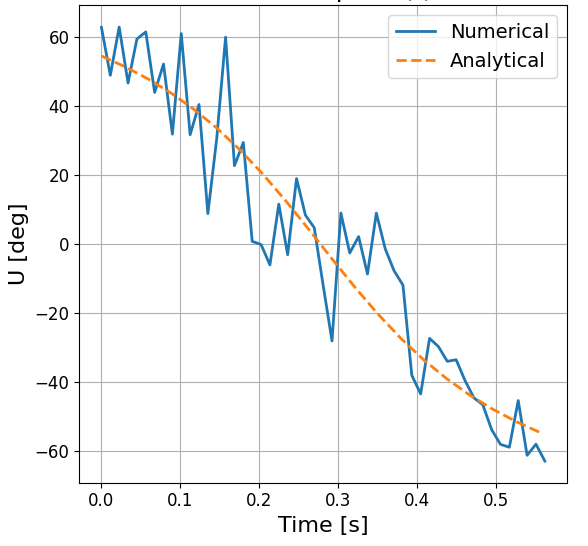
\includegraphics[keepaspectratio]{Chapter2_imgs/hs_state.png}}

}

\subcaption{\label{fig-ch2-hs-state}State variables
\(\tilde{\mathbf{x}}_1, \tilde{\mathbf{x}}_2, \tilde{\mathbf{x}}_3, \tilde{\mathbf{x}}_4\)}

\end{minipage}%
%
\begin{minipage}[t]{0.50\linewidth}

\centering{

\pandocbounded{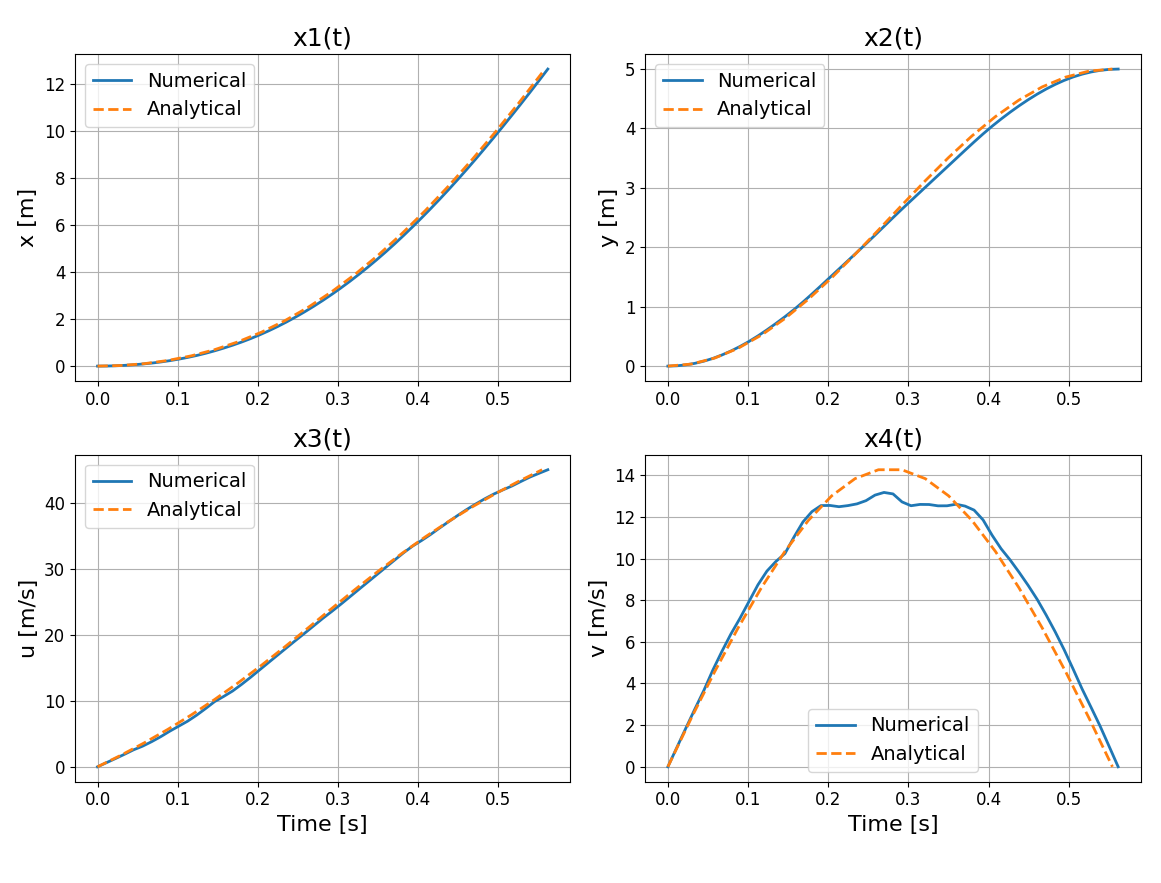
\includegraphics[keepaspectratio]{Chapter2_imgs/hs_control.png}}

}

\subcaption{\label{fig-ch2-hs-control}Control input
\(\mathbf{\tilde{u}}\)}

\end{minipage}%

\caption{\label{fig-ch2-hs-solution}Numerical solution of the LTS
problem using the H-S method.}

\end{figure}%

Similar to last method, MSE is computed for each state variable and the
control input and, error in the final time.

\begin{longtable}[]{@{}lr@{}}
\caption{Computed MSE values and final time comparison using the
Hermite--Simpson method}\label{tbl-ch2-mse-hs}\tabularnewline
\toprule\noalign{}
Quantity & Value \\
\midrule\noalign{}
\endfirsthead
\toprule\noalign{}
Quantity & Value \\
\midrule\noalign{}
\endhead
\bottomrule\noalign{}
\endlastfoot
\(\text{MSE}(x_1)\) & \(3.6200 \times 10^{-3}\) \\
\(\text{MSE}(x_2)\) & \(1.9110 \times 10^{-3}\) \\
\(\text{MSE}(x_3)\) & \(8.6762 \times 10^{-2}\) \\
\(\text{MSE}(x_4)\) & \(4.5058 \times 10^{-1}\) \\
\(\text{MSE}(u)\) & \(1.6727 \times 10^{2}\) \\
\(t_f^{\text{num}}\) & \(0.5617 \, \text{s}\) \\
\(\varepsilon_{t_f}\) & \(7.1137 \times 10^{-3} \, \text{s}\) \\
\end{longtable}

To alleviate this issue and promote smoother control profiles, a
regularization term can be added to the cost functional. This term
penalizes the rate of change in the control input and helps suppress
high-frequency oscillations, thereby improving numerical stability and
producing more realistic control behavior.

\subsection{Regularization Strategies for Control
Smoothing}\label{regularization-strategies-for-control-smoothing}

To promote smoother control profiles and mitigate undesirable
oscillations (chattering) in control inputs, a regularization term
\citep{sanchez2016optimal} is often added to the objective function.
This term penalizes large variations in the control trajectory by
discouraging abrupt changes in the derivative of the control vector
\(\mathbf{\tilde{u}}\). Such an approach is particularly useful in
trajectory optimization problems, where noisy or highly oscillatory
controls can be both unrealistic and numerically unstable.

The regularization cost is computed using a second-order finite
difference approximation of the first derivative of the control input.
Note that the time step \(\Delta t\) is omitted from the formulation.

\textbf{Regularization Term}

A central difference approximation is used for all interior nodes
\(i = 0, \dots, N\):

\begin{equation}\protect\phantomsection\label{eq-ch2-central-diff-reg}{
R(\mathbf{\tilde{u}}) = \sum_{i=0}^{N} \left( \frac{\mathbf{{u}}_{i+1} - \mathbf{u}_{i-1}}{2} \right)^2
}\end{equation}

\textbf{Boundary Approximations}

At the boundaries where central differences are not applicable,
second-order forward and backward differences are used:

\begin{equation}\protect\phantomsection\label{eq-ch2-forward-diff}{
\text{First Point } (i = 0): \quad \left( \frac{-3\mathbf{u}_0 + 4\mathbf{u}_1 - \mathbf{u}_2}{2} \right)^2
}\end{equation}

\begin{equation}\protect\phantomsection\label{eq-ch2-backward-diff}{
\text{Last Point } (i = N): \quad \left( \frac{3\mathbf{u}_{N} - 4\mathbf{u}_N + \mathbf{u}_{N-1}}{2} \right)^2
}\end{equation}

\textbf{Regularized Objective Function}

The modified objective function incorporating the regularization term
is:

\begin{equation}\protect\phantomsection\label{eq-ch2-reg-objective}{
J' = J + \beta R(\mathbf{\tilde{u}})
}\end{equation}

where \(J\) is the original objective function (e.g., final time or
control effort), \(R(\mathbf{\tilde{u}})\) is the regularization term,
and \(\beta\) is a user-defined weighting parameter that balances
optimality and smoothness.

Including this regularization term reduces high-frequency content in the
control signal \(\mathbf{u}\), thereby suppressing chattering and
enhancing the numerical stability and physical plausibility of the
computed solution.

\subsubsection{Application to the LTS
Problem}\label{application-to-the-lts-problem}

To enhance the smoothness of the control input in the LTS (LTS) problem,
a regularization term \(J_{\text{reg}}\) is added to the objective
function. This penalizes abrupt variations in the control trajectory
\(\mathbf{\tilde{u}}\), reducing high-frequency oscillations and
producing a more realistic control profile.

The modified objective function is defined as:

\begin{equation}\protect\phantomsection\label{eq-ch2-regularized-obj}{
J' = t_f + \beta \, R(\mathbf{\tilde{u}}),
}\end{equation}

where \(t_f\) denotes the final time, and \(\beta = 10^{-5}\) is the
regularization parameter. The term \(\mathbf{\tilde{u}}\) represents the
discretized control inputs. The discretization step \(\Delta t\) is
omitted in the formulation, as it is effectively absorbed into the
regularization weight \(\beta\). Based on findings in the
literature\textasciitilde{}\citep{sanchez2016optimal}, a value of
\(\beta = 10^{-5}\) has been shown to effectively suppress chattering in
the control signal.

\subsubsection{Effect of Regularization Weight and Optimizer
Choice}\label{effect-of-regularization-weight-and-optimizer-choice}

To improve control smoothness in the LTS problem, both the
regularization weight \(\beta\) and the choice of optimization algorithm
were evaluated. The H-S collocation method was used with different
values of \(\beta\), keeping the overall numerical setup unchanged.

\begin{figure}

\begin{minipage}[t]{0.50\linewidth}

\centering{

\pandocbounded{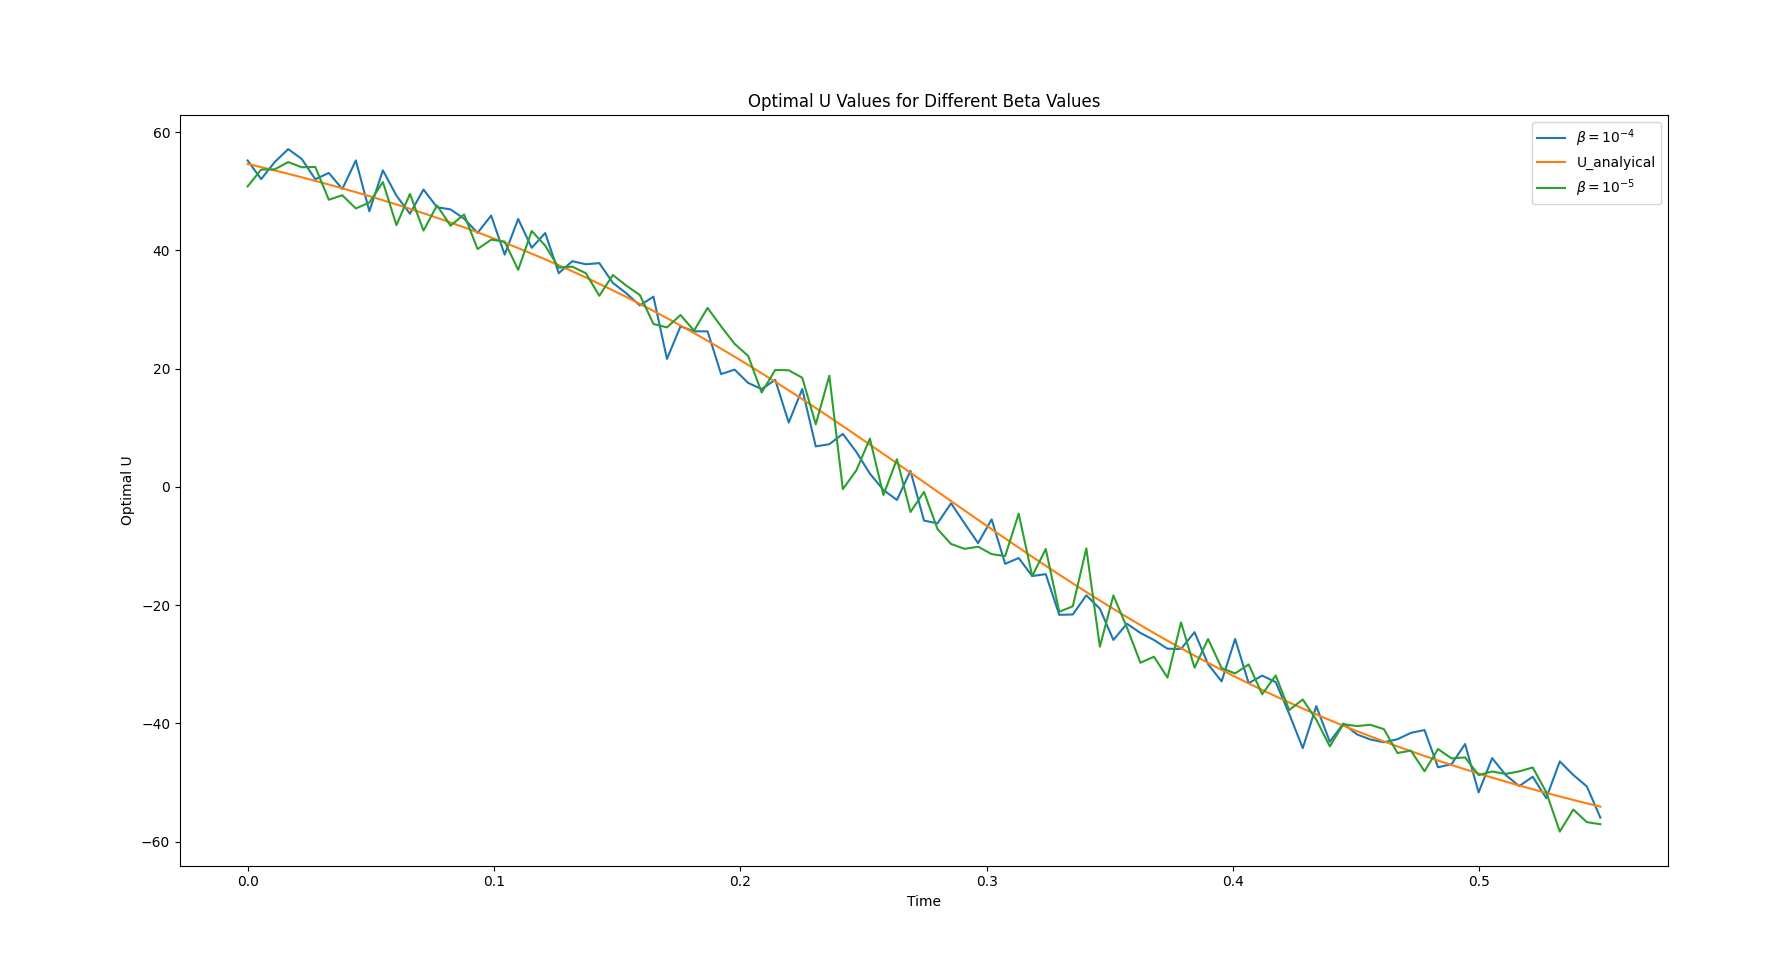
\includegraphics[keepaspectratio]{Chapter2_imgs/U_opt_diff_beta_values.PNG}}

}

\subcaption{\label{fig-ch2-u-beta-variation}Effect of varying \(\beta\)
on \(\mathbf{\tilde{u}}\)}

\end{minipage}%
%
\begin{minipage}[t]{0.50\linewidth}

\centering{

\pandocbounded{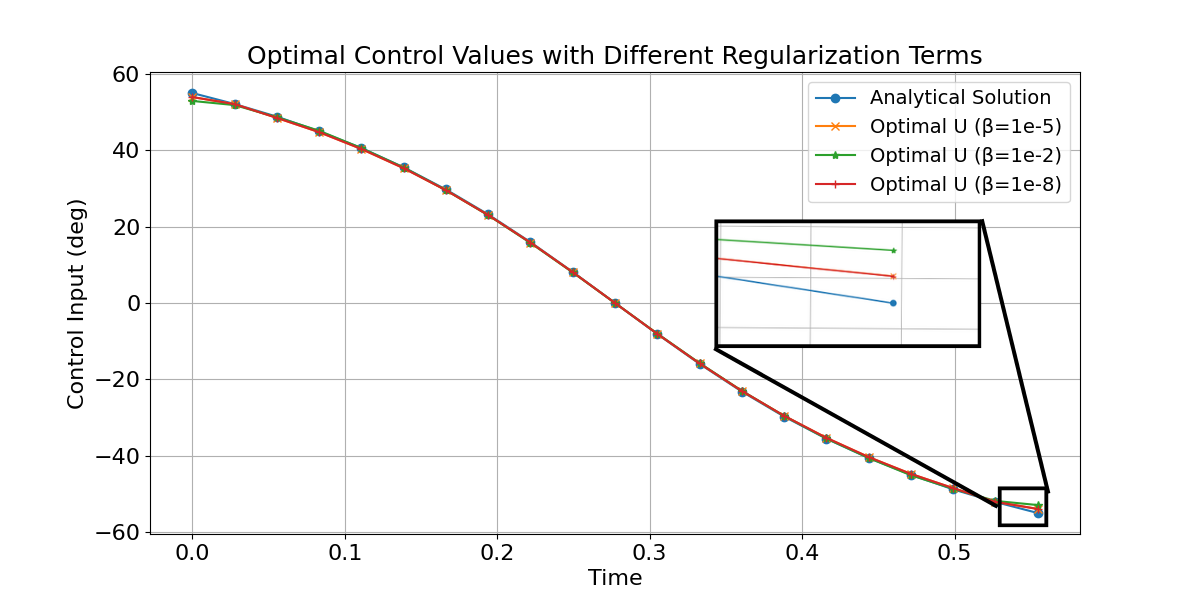
\includegraphics[keepaspectratio]{Chapter2_imgs/var_beta_U_opt_zoom.png}}

}

\subcaption{\label{fig-ch2-u-optimizer-variation}Effect of optimizer
choice on \(\mathbf{\tilde{u}}\)}

\end{minipage}%

\caption{\label{fig-ch2-reg-results}Comparison of control input
\(\mathbf{u}(t)\) under varying regularization weights and optimization
algorithms.}

\end{figure}%

As shown in Figure~\ref{fig-ch2-reg-results}(a), increasing the
regularization weight \(\beta\) results in progressively smoother
control trajectories. The regularization term penalizes large variations
in the control input and helps suppress chattering, although some
high-frequency artifacts persist due to the underlying bang-bang nature
of the optimal solution. This highlights the difficulty of approximating
discontinuous control laws using smooth polynomial-based collocation
methods alone.

As shown in Figure~\ref{fig-ch2-reg-results}(b), the use of different
\(\beta\) values with the trust-region method results in smoother
control profiles. Although slight variations can be observed near the
boundaries, the control profile corresponding to \(\beta = 10^{-5}\)
aligns almost perfectly with the analytical solution, making it the most
suitable choice for this problem.

Unlike some solvers like SLSQP, which can get stuck in poor local
minima, the trust-region method is more effective at exploring the
entire solution space. It avoids premature convergence and increases the
chances of finding better, or even globally optimal, solutions. This
makes it particularly suitable for problems like the LTS, which involve
sharp control transitions and complex dynamics.

When combined with the H-S method and an appropriate regularization
term, the trust-region method results in smoother and more accurate
trajectories. The final optimized states and control are shown in
Figure~\ref{fig-ch2-final-reg}. The improved solution exhibits reduced
numerical artifacts, excellent stability, and a closer match to the
ideal bang-bang structure.

\begin{figure}

\begin{minipage}[t]{0.50\linewidth}

\centering{

\pandocbounded{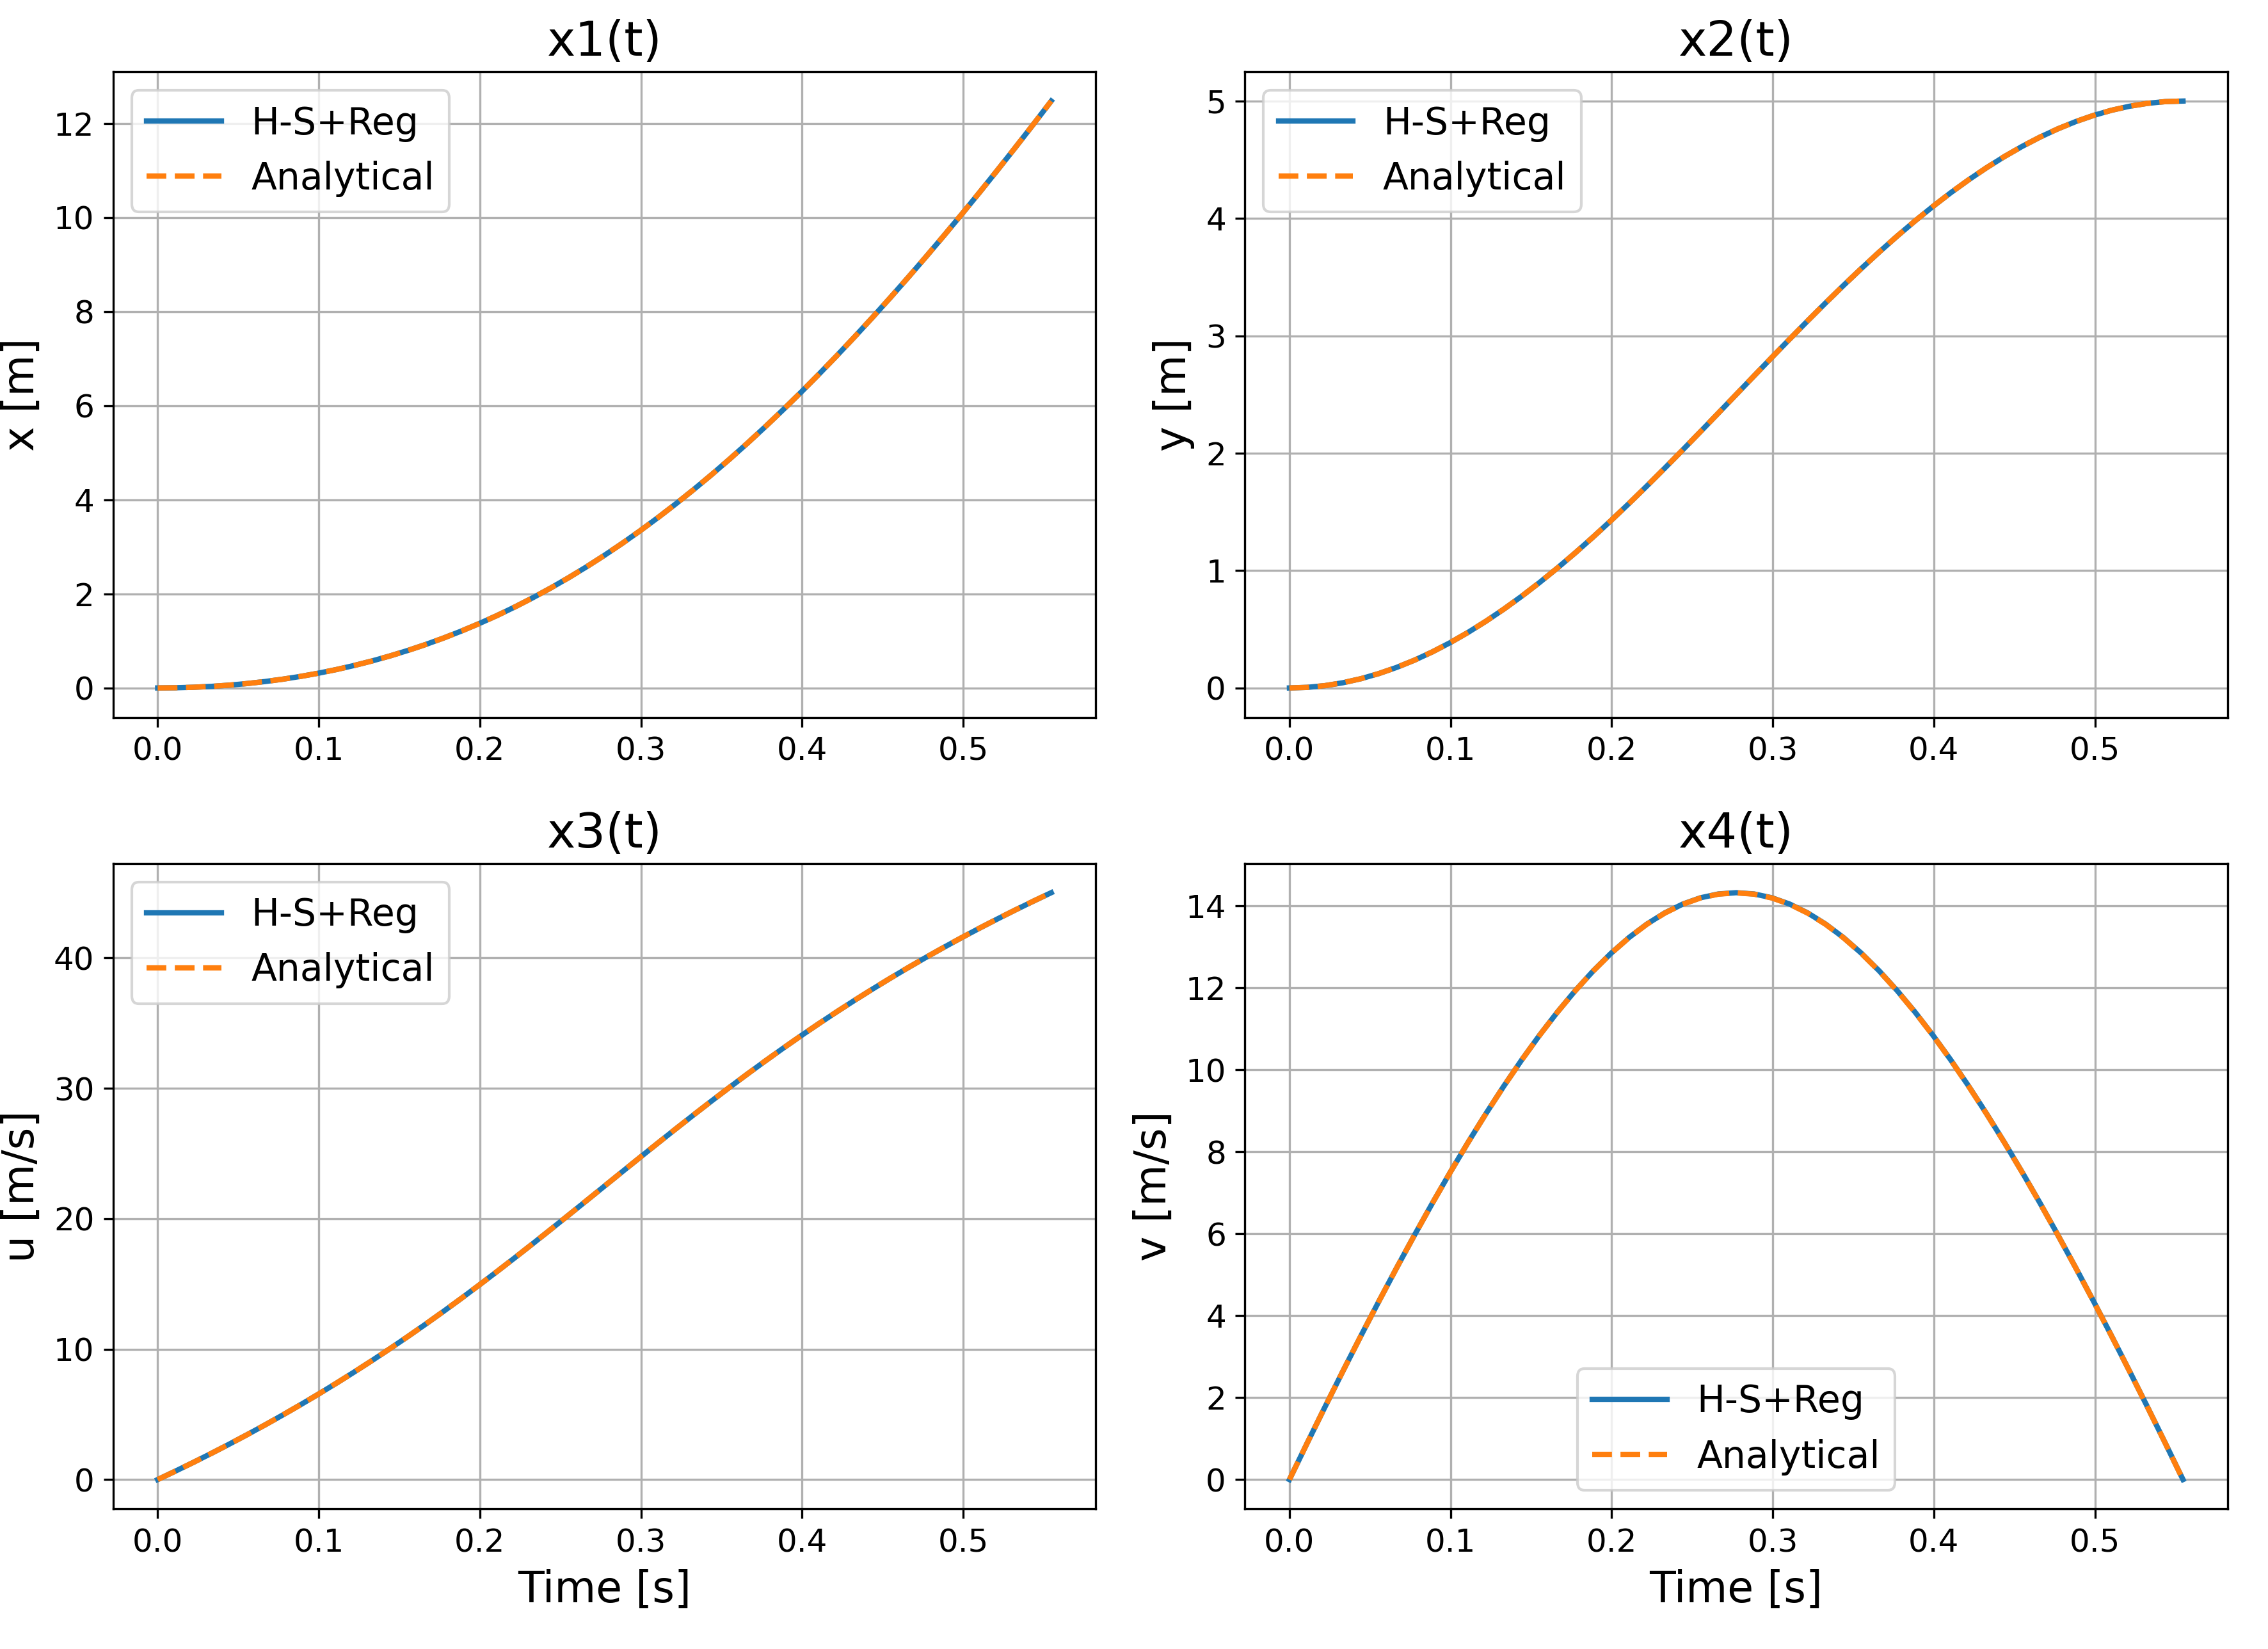
\includegraphics[keepaspectratio]{Chapter2_imgs/state_reg.png}}

}

\subcaption{\label{fig-ch2-state-reg}State variables
\({x}_1, {x}_2, {x}_3, {x}_4\)}

\end{minipage}%
%
\begin{minipage}[t]{0.50\linewidth}

\centering{

\pandocbounded{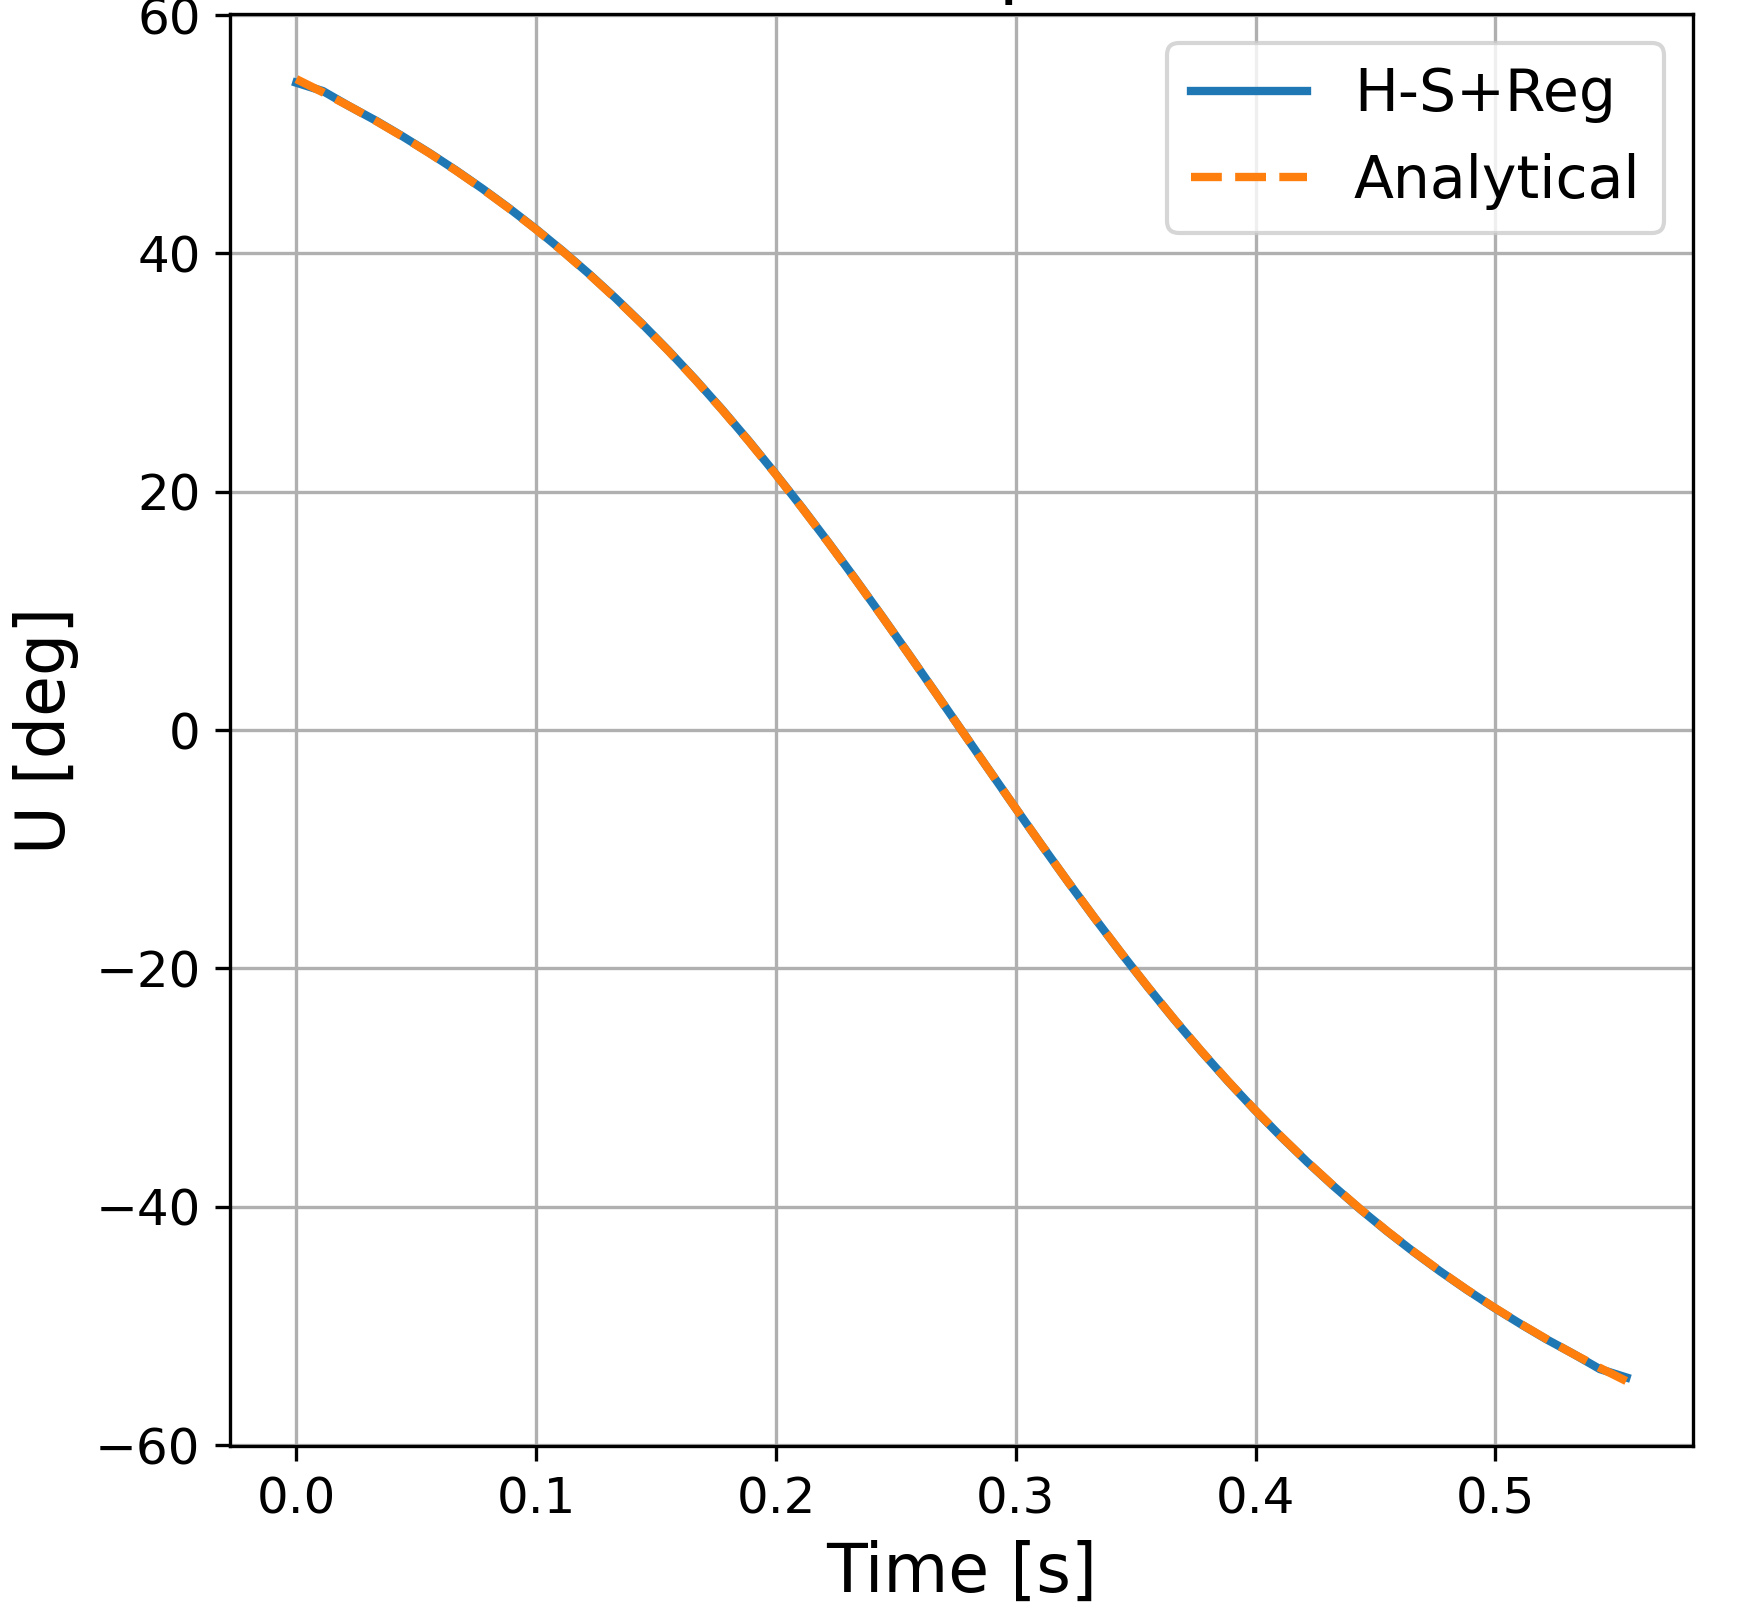
\includegraphics[keepaspectratio]{Chapter2_imgs/control_reg.png}}

}

\subcaption{\label{fig-ch2-control-reg}Smoothed control input
\(\mathbf{\tilde{u}}(t)\)}

\end{minipage}%

\caption{\label{fig-ch2-final-reg}Final optimized trajectories using
Hermite--Simpson method, regularization, and trust-region optimizer.}

\end{figure}%

\begin{longtable}[]{@{}lr@{}}
\caption{Computed MSE values and final time comparison using the
regularized objective}\label{tbl-ch2-mse-reg}\tabularnewline
\toprule\noalign{}
Quantity & Value \\
\midrule\noalign{}
\endfirsthead
\toprule\noalign{}
Quantity & Value \\
\midrule\noalign{}
\endhead
\bottomrule\noalign{}
\endlastfoot
\(\text{MSE}(x_1)\) & \(1.0000 \times 10^{-6}\) \\
\(\text{MSE}(x_2)\) & \(1.7240 \times 10^{-3}\) \\
\(\text{MSE}(x_3)\) & \(3.1893 \times 10^{-3}\) \\
\(\text{MSE}(x_4)\) & \(8.3461 \times 10^{-3}\) \\
\(\text{MSE}(\mathbf{\tilde{u}})\) & \(4.3790 \times 10^{-3}\) \\
\(t_f^{*}\) & \(0.5546 \, \text{s}\) \\
\(\varepsilon_{t_f}\) & \(4.8597 \times 10^{-5} \, \text{s}\) \\
\end{longtable}

These results confirm that the combined use of regularization and the
trust-region method significantly improves both the smoothness and the
numerical accuracy of the computed control and state trajectories.

\subsubsection{Limitations of Transcription-Based
Approaches}\label{limitations-of-transcription-based-approaches}

Direct transcription methods, especially when enhanced with
regularization and robust optimizers, offer practical and reliable
solutions for complex trajectory optimization problems. However, they
have inherent limitations. Direct transcription approximates state and
control trajectories numerically, which can lead to accuracy loss near
discontinuities such as bang-bang switches \citep{sanchez2018real}.
Moreover, direct methods do not explicitly expose the necessary
conditions for optimality, limiting analytical insight.

Direct collocation methods, such as the Hermite-Simpson scheme discussed
previously, improve stability by enforcing dynamics at multiple points
but may require dense discretization to achieve high accuracy,
increasing computational cost \citep{rao2010survey}.

These limitations motivate an alternative formulation in which the
necessary conditions for optimality are derived analytically and solved
numerically. This is the basis of the indirect method presented in the
next section, where the optimal control problem is recast as a two-point
boundary value problem (TPBVP) using the Pontryagin Maximum Principle
(PMP).

\subsection{Pontryagin Maximum Principle and the TPBVP
Formulation}\label{pontryagin-maximum-principle-and-the-tpbvp-formulation}

The indirect formulation for solving trajectory optimization problems is
grounded in optimal control theory, particularly the calculus of
variations and Pontryagin's Maximum Principle (PMP)
\citep{sanchez2018real}. This approach transforms the trajectory
optimization problem into a boundary value problem (BVP) by deriving
necessary conditions for optimality. The TPBVP that results from this
transformation is also the formulation later solved using
Physics-Informed Neural Networks in Chapter 3, and is therefore
developed in detail here.

\subsubsection{Problem Formulation}\label{problem-formulation}

Consider a general trajectory optimization problem defined over the time
interval \([t_0, t_f]\), where the objective is to minimize a
performance index consisting solely of a Lagrangian term:

\begin{equation}\protect\phantomsection\label{eq-ch2-cost-function}{
\min_{\mathbf{u}(t), \mathbf{x}(t)} \quad J = \int_{t_0}^{t_f} L(\mathbf{x}(t), \mathbf{u}(t), t) \, dt,
}\end{equation}

subject to the system dynamics:

\begin{equation}\protect\phantomsection\label{eq-ch2-dynamics}{
\dot{\mathbf{x}}(t) = \mathbf{f}(\mathbf{x}(t), \mathbf{u}(t), t),
}\end{equation}

and the boundary conditions:

\begin{equation}\protect\phantomsection\label{eq-ch2-bc-indirect}{
\mathbf{x}(t_0) = \mathbf{x}_0, \quad \mathbf{x}(t_f) = \mathbf{x}_f.
}\end{equation}

\subsubsection{Application of the Pontryagin Maximum
Principle}\label{application-of-the-pontryagin-maximum-principle}

To derive the necessary conditions for optimality, we begin by defining
the Hamiltonian function \citep{pinch1995optimal}:

\begin{equation}\protect\phantomsection\label{eq-ch2-hamiltonian}{
H(\mathbf{x}, \mathbf{u}, \boldsymbol{\lambda}, t) = L(\mathbf{x}, \mathbf{u}, t) + \boldsymbol{\lambda}^\top \mathbf{f}(\mathbf{x}, \mathbf{u}, t),
}\end{equation}

where \(\boldsymbol{\lambda}(t) \in \mathbb{R}^n\) is the costate
vector, having the same dimension as the state vector \(\mathbf{x}(t)\).

\textbf{Optimal Control Law.} According to the Pontryagin Maximum
Principle (PMP), the optimal control \(\mathbf{u}^*(t)\) minimizes the
Hamiltonian at every instant:

\begin{equation}\protect\phantomsection\label{eq-ch2-optimal-control}{
\mathbf{u}^*(t) = \arg\min_{\mathbf{u}} H(\mathbf{x}(t), \mathbf{u}, \boldsymbol{\lambda}(t), t).
}\end{equation}

A necessary condition for optimality is that the Hamiltonian is
stationary with respect to the control input:

\begin{equation}\protect\phantomsection\label{eq-ch2-control-stationarity}{
\frac{\partial H}{\partial \mathbf{u}} = 0.
}\end{equation}

Solving this stationarity condition yields an explicit or implicit
expression for the optimal control \(\mathbf{u}^*(t)\) as a function of
\(\mathbf{x}(t)\), \(\boldsymbol{\lambda}(t)\), and \(t\).

\textbf{State and Costate Dynamics.} Once the optimal control law
\(\mathbf{u}^*(t)\) is obtained, it is substituted back into the system
to define a boundary value problem involving the state and costate
trajectories. The dynamics of these variables are given by:

\begin{equation}\protect\phantomsection\label{eq-ch2-state-dynamics}{
\dot{\mathbf{x}}(t) = \frac{\partial H}{\partial \boldsymbol{\lambda}} = \mathbf{f}(\mathbf{x}, \mathbf{u}^*, t) \tag{State dynamics}
}\end{equation}

\begin{equation}\protect\phantomsection\label{eq-ch2-costate-dynamics}{
\dot{\boldsymbol{\lambda}}(t) = -\frac{\partial H}{\partial \mathbf{x}} \tag{Costate dynamics}
}\end{equation}

These equations are typically coupled and nonlinear, and must be solved
simultaneously.

\textbf{Transversality Conditions.} To solve the state-costate system as
a boundary value problem, appropriate terminal conditions are required.
These are provided by the transversality conditions:

\begin{itemize}
\tightlist
\item
  If a terminal cost \(\Phi(\mathbf{x}(t_f))\) is present in the
  objective, then:
\end{itemize}

\begin{equation}\protect\phantomsection\label{eq-ch2-costate-boundary}{
\boldsymbol{\lambda}(t_f) = \frac{\partial \Phi}{\partial \mathbf{x}(t_f)}.
}\end{equation}

\begin{itemize}
\tightlist
\item
  If the terminal state \(\mathbf{x}(t_f)\) is free (i.e., not
  constrained), the costate at final time must satisfy:
\end{itemize}

\begin{equation}\protect\phantomsection\label{eq-ch2-free-terminal-state}{
\boldsymbol{\lambda}(t_f) = \mathbf{0}.
}\end{equation}

\begin{itemize}
\tightlist
\item
  If the final time \(t_f\) is free (as in time-optimal problems), the
  Hamiltonian must satisfy:
\end{itemize}

\begin{equation}\protect\phantomsection\label{eq-ch2-free-final-time}{
H(t_f) = 0.
}\end{equation}

\textbf{Optimality System.} The complete optimality system consists of:

\begin{itemize}
\tightlist
\item
  The state equations (Equation~\ref{eq-ch2-state-dynamics}) with
  initial condition \(\mathbf{x}(t_0) = \mathbf{x}_0\),
\item
  The costate equations (Equation~\ref{eq-ch2-costate-dynamics}) with
  terminal boundary condition from the transversality condition,
\item
  The optimal control law \(\mathbf{u}^*(t)\) obtained from solving
  (Equation~\ref{eq-ch2-control-stationarity}).
\end{itemize}

This boundary value problem can be solved using numerical techniques
such as the shooting method or collocation-based approaches. The system
must be integrated forward in time for the state and backward for the
costate, with iterations to satisfy all boundary conditions.

\subsubsection{Solving the Boundary Value
Problem}\label{solving-the-boundary-value-problem}

The system of first-order differential equations formed by the state
dynamics, costate dynamics, and optimal control law constitutes a TPBVP.
These equations are solved numerically using methods such as shooting
techniques or collocation methods.

The indirect method provides high accuracy since it directly enforces
the necessary conditions for optimality. However, it faces several
limitations in practical implementation. One major drawback is its
sensitivity to the initial guess; solving the resulting boundary value
problem (BVP) requires accurate initialization of both state and costate
variables, and poor guesses often result in divergence or convergence to
suboptimal solutions \citep{sanchez2018real}. Additionally, the BVP is
often numerically stiff, especially in problems involving highly
nonlinear or high-dimensional dynamics, which can make shooting methods
unstable and sensitive to perturbations.

The system of ODEs for the state and costate variables, along with the
associated boundary conditions, can also be solved using advanced
machine learning techniques such as Physics-Informed Neural Networks
(PINNs). PINNs leverage deep learning to approximate the solution to
differential equations \citep{raissi2019physics} by incorporating the
governing physical laws (in this case, the system dynamics and costate
equations) directly into the training process, which is explored in the
next chapter.

\newpage

\section{Trajectory Optimization using Deep Neural
Network}\label{trajectory-optimization-using-deep-neural-network}

This chapter applies Physics-Informed Neural Networks (PINNs) to
trajectory optimization problems. It begins with a general formulation
of the PINN framework, then applies it progressively to a scalar
benchmark problem, the classical Linear Tangent Steering (LTS) problem,
and finally to a class of parameterized trajectory optimization problems
in which many problem instances must be solved efficiently. The chapter
closes with a physics-informed simplification that exploits known
solution structure, and a discussion of remaining limitations.

\subsection{Physics-Informed Neural Networks
Architecture}\label{physics-informed-neural-networks-architecture}

Physics-Informed Neural Networks (PINNs) are a class of deep learning
models designed to solve ordinary and partial differential equations
(ODEs and PDEs) by incorporating physical laws directly into the neural
network training process. Unlike traditional numerical methods that rely
on mesh-based discretization, PINNs embed the governing equations as
soft constraints into the loss function, enabling mesh-free,
data-efficient, and interpretable solutions
\citep{raissi2019physics, karniadakis2021physics}.

The key idea behind PINNs is to construct a neural network that
approximates the solution to a differential equation while minimizing a
composite loss function. This loss typically includes two components:
(i) the residuals of the governing equations, which enforce the physical
constraints, and (ii) the error at initial and boundary conditions. By
training the network to reduce these terms simultaneously, PINNs produce
solutions that respect both data and physics.

PINNs offer significant advantages in solving complex and
high-dimensional problems in fields such as fluid dynamics, heat
conduction, elasticity, and optimal control \citep{cuomo2022scientific}.
Their ability to encode prior knowledge in the form of differential
operators improves generalization and stability, especially when
observational data are sparse or noisy. Recent advances have extended
PINNs to handle stiff systems, multi-physics problems, and inverse
modeling tasks, showcasing their versatility and growing importance in
scientific computing \citep{wang2021understanding, mao2020physics}.
Furthermore, innovations in adaptive activation functions, domain
decomposition, and transfer learning continue to enhance their accuracy
and scalability \citep{mcclenny2020self, shukla2021parallel}.

\subsubsection{PINN Formulation}\label{pinn-formulation}

Consider a general first-order system of ordinary differential equations
given by:

\begin{equation}\protect\phantomsection\label{eq-ch3-pinn-ode}{
\dot{\mathbf{x}}(t) = \mathbf{f}(\mathbf{x}(t), t), \quad t \in [0, t_f],
}\end{equation}

where \(\mathbf{x}(t) \in \mathbb{R}^n\) is the state vector, and
\(\mathbf{f} : \mathbb{R}^n \times \mathbb{R} \rightarrow \mathbb{R}^n\)
is a known (possibly nonlinear) function describing the system dynamics.
The system is subject to an initial condition:

\begin{equation}\protect\phantomsection\label{eq-ch3-pinn-ic}{
\mathbf{x}(0) = \mathbf{x}_0.
}\end{equation}

In the PINN framework, the solution \(\mathbf{x}(t)\) is approximated by
a neural network \(\mathbf{x}_{\theta}(t)\), where \(\theta\) represents
the trainable parameters of the network.

\subsubsection{Loss Function of PINNs}\label{loss-function-of-pinns}

The total loss function used to train the PINN is composed of two terms:
the residual loss and the initial condition loss. It is defined as:

\begin{equation}\protect\phantomsection\label{eq-ch3-pinn-loss}{
\mathcal{L}_{\text{PINN}} = \omega_1 \mathcal{L}_{\text{residual}} + \omega_2 \mathcal{L}_{\text{IC}},
}\end{equation}

where \(\omega_1\) and \(\omega_2\) are weighting coefficients that
balance the enforcement of the system dynamics and the initial
condition, where \(\sum_{i=0}^{N}\omega_i = 1\)

The residual loss is computed over a set of \(N\) collocation points
\(\{t_i\}_{i=1}^{N} \subset [0, t_f]\):

\begin{equation}\protect\phantomsection\label{eq-ch3-residual-loss}{
\mathcal{L}_{\text{residual}} = \frac{1}{N} \sum_{i=1}^{N} \left\| \frac{d}{dt} \mathbf{x}_{\theta}(t_i) - \mathbf{f}(\mathbf{x}_{\theta}(t_i), t_i) \right\|^2.
}\end{equation}

The initial condition loss ensures that the predicted trajectory starts
at the correct initial value:

\begin{equation}\protect\phantomsection\label{eq-ch3-ic-loss}{
\mathcal{L}_{\text{IC}} = \left\| \mathbf{x}_{\theta}(0) - \mathbf{x}_0 \right\|^2.
}\end{equation}

This formulation ensures that the learned function
\(\mathbf{x}_{\theta}(t)\) adheres to both the physics (via the ODE
residual) and the given initial condition.

\subsubsection{Network Architecture}\label{network-architecture}

A typical PINN architecture consists of:

\begin{itemize}
\tightlist
\item
  \textbf{Input Layer:} Receives input variables such as time, spatial
  coordinates, or parameters.
\item
  \textbf{Hidden Layers:} Multiple fully connected layers using
  nonlinear activation functions such as Tanh or ReLU to learn the
  functional mapping.
\item
  \textbf{Output Layer:} Produces the predicted solution
  \(\mathbf{x}_{\theta}(t) \in \mathbb{R}^n\).
\end{itemize}

This architecture is flexible and can be adapted to accommodate multiple
outputs, complex nonlinearities, or additional inputs such as control
parameters or auxiliary variables.

\subsubsection{Training Procedure}\label{training-procedure}

Training a PINN involves minimizing the loss function
\(\mathcal{L}_{\text{PINN}}\) using gradient-based optimization methods
such as stochastic gradient descent (SGD) or Adam. The time derivatives
of the neural network outputs are computed via automatic
differentiation. During each iteration, gradients of the loss with
respect to the network parameters \(\theta\) are computed and used to
update the model. The goal is to simultaneously minimize the equation
residuals and enforce the boundary/initial conditions.

\begin{figure}

\centering{

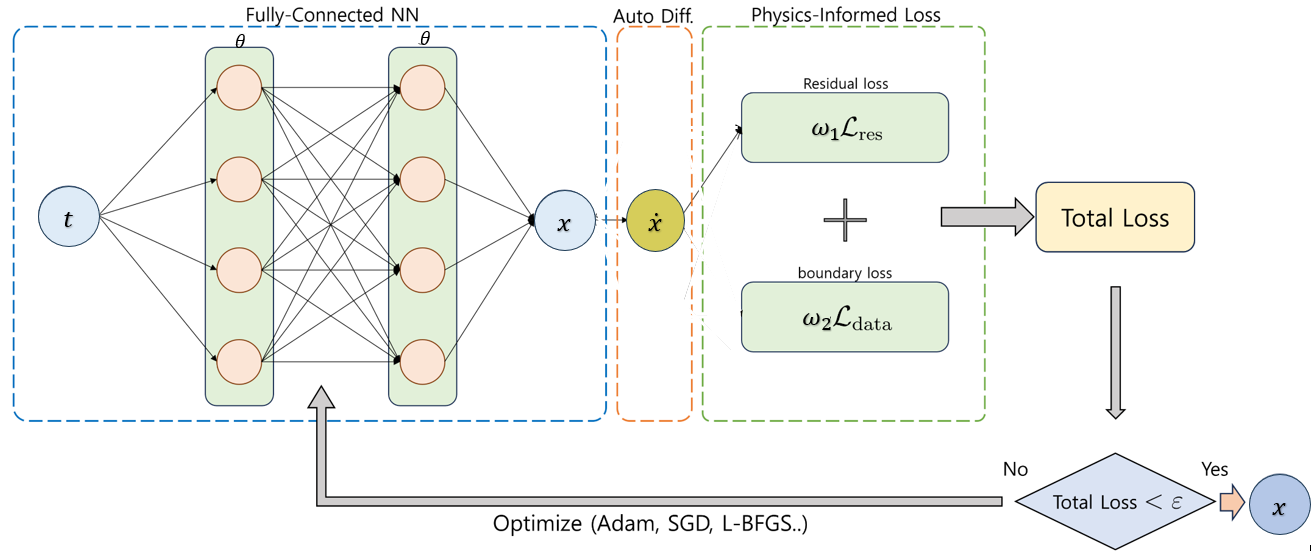
\includegraphics[width=0.75\linewidth,height=\textheight,keepaspectratio]{Chapter3_imgs/pinn_model.PNG}

}

\caption{\label{fig-ch3-pinn-architecture}PINNs architecture
\citep{cuomo2022scientific}}

\end{figure}%

\subsubsection{Solving Coupled ODEs}\label{solving-coupled-odes}

Coupled ODE systems frequently appear in scientific and engineering
contexts such as trajectory optimization, chemical kinetics and
multi-body dynamics. These systems consist of multiple interdependent
differential equations that must be solved simultaneously.

PINNs handle coupled systems by using a NN with multiple outputs
corresponding to each component of the state vector. The residuals of
all coupled equations are computed and minimized together, while initial
or boundary conditions for each state variable are incorporated into the
loss function. This approach enables the network to learn solutions that
satisfy the entire coupled system consistently.

\subsubsection{Advantages and
Challenges}\label{advantages-and-challenges}

PINNs offer several advantages. By embedding prior physical knowledge,
PINNs significantly reduce the need for large labeled datasets, thereby
improving data efficiency
\citep{raissi2019physics, karniadakis2021physics}. Moreover, the
solutions produced are physically consistent, which enhances
generalization, even in regions beyond the training data
\citep{cuomo2022scientific}. Another key benefit is their mesh-free
nature, eliminating the need for mesh generation or discretization,
which simplifies implementation for complex geometries
\citep{raissi2019physics}.

Despite these benefits, several challenges remain. Training PINNs for
stiff or highly nonlinear systems often suffers from gradient imbalance
and instability, which can impede convergence
\citep{wang2021understanding, lu2021deepxde}. Additionally, selecting
appropriate weighting factors for different loss components, such as
residual and boundary condition losses, is nontrivial and can
significantly affect performance \citep{mcclenny2020self}. The
computational cost is another consideration, as training deep neural
networks with automatic differentiation can be resource-intensive and
time-consuming \citep{shukla2021parallel}.

Recent advances have addressed some of these challenges through methods
such as adaptive activation functions, residual-based adaptive sampling,
transfer learning, and domain decomposition, which improve training
stability and efficiency
\citep{mcclenny2020self, shukla2021parallel, lu2021deepxde}.

\subsection{Solving ODEs using PINNs}\label{solving-odes-using-pinns}

This section applies the PINN framework to specific trajectory
optimization problems. Two examples are considered: a scalar
linear-quadratic benchmark taken from optimal control theory, and the
classical Linear Tangent Steering (LTS) problem introduced in
Section~\ref{sec-ch2-lts}. Each example is presented end-to-end ---
problem statement, PINN representation, loss function, training setup,
and baseline result --- so that the reader can follow a complete
workflow without jumping between sections.

\subsubsection{Scalar Trajectory Optimization
Problem}\label{scalar-trajectory-optimization-problem}

We first consider an optimal control problem given in
\citep{pinch1995optimal} (Example 4.3), involving a linear first-order
dynamical system in which the state \(x(t)\) evolves according to the
control input \(u(t)\) through the relation
\(\dot{x}(t) = -x(t) + u(t)\). The goal is to drive the system from the
initial condition \(x(0) = 0\) to the final state \(x(1) = 2\) over the
fixed time interval \(t \in [0, 1]\), while determining the optimal
control \(u(t)\) that minimizes the quadratic cost functional penalizing
both the magnitude of the state and the control effort. This cost
functional captures the trade-off between maintaining the state close to
the origin and minimizing the energy or effort required for control.

The system dynamics, boundary conditions, and cost functional are:

\begin{equation}\protect\phantomsection\label{eq-ch3-scalar-problem}{
\begin{aligned}
\dot{x}(t) &= -x(t) + u(t), && \text{(System dynamics)} \\
x(0) &= 0, \quad x(1) = 2, && \text{(Boundary conditions)} \\
J &= \frac{1}{2} \int_0^1 \left( 3x^2(t) + u^2(t) \right) \, dt. && \text{(Cost functional)}
\end{aligned}
}\end{equation}

\textbf{Analytical reduction via PMP.} The Hamiltonian is

\begin{equation}\protect\phantomsection\label{eq-ch3-scalar-hamiltonian}{
H = \frac{3}{2} x^2 + \frac{1}{2} u^2 + \lambda (-x + u).
}\end{equation}

There is no constraint on \(u\), so to maximize \(H\) we consider
\(\frac{\partial H}{\partial u}\):

\begin{equation}\protect\phantomsection\label{eq-ch3-scalar-hu}{
\frac{\partial H}{\partial u} = -u + \lambda \quad \text{and} \quad \frac{\partial^2 H}{\partial u^2} = -1.
}\end{equation}

So \(H\) is maximized when \(u = \lambda\) and the corresponding state
equation is

\begin{equation}\protect\phantomsection\label{eq-ch3-scalar-state-ode}{
\dot{x} = -x + \lambda
}\end{equation}

and \(\lambda\) satisfies

\begin{equation}\protect\phantomsection\label{eq-ch3-scalar-costate-ode}{
\dot{\lambda} = -\frac{\partial H}{\partial x} = 3x + \lambda.
}\end{equation}

Thus, \(\ddot{x} = 4x\) and \(\lambda = \dot{x} + x\), giving

\begin{equation}\protect\phantomsection\label{eq-ch3-scalar-x-sol}{
x = A \sinh(2t + \alpha)
}\end{equation}

and

\begin{equation}\protect\phantomsection\label{eq-ch3-scalar-lambda}{
\lambda = u^* = A\left(2 \cosh(2t + \alpha) + \sinh(2t + \alpha)\right).
}\end{equation}

The end conditions on \(x\) give \(\alpha = 0\) and \(A = 2/\sinh 2\).
Thus, the optimal control is

\begin{equation}\protect\phantomsection\label{eq-ch3-scalar-u-optimal}{
u^* = \frac{2(2 \cosh 2t + \sinh 2t)}{\sinh 2}.
}\end{equation}

\textbf{PINN representation and loss.} Using the optimality relations
derived above, the system to be learned by the PINN reduces to the
coupled state--costate ODEs:

\begin{equation}\protect\phantomsection\label{eq-ch3-scalar-state-costate}{
\begin{aligned}
\dot{x}(t) &= -x(t) + \lambda(t), && \text{(State ODE)}\\
\dot{\lambda}(t) &= 3x(t) + \lambda(t), && \text{(Costate ODE)}\\
\end{aligned}
}\end{equation}

In the PINN framework, the state and costate equations are enforced
through a loss that penalizes both the ODE residuals and the boundary
conditions.

\textbf{Residual Loss.}

\begin{equation}\protect\phantomsection\label{eq-ch3-scalar-residual}{
\mathcal{L}_{\text{residual}} = \frac{1}{N} \sum_{i=1}^{N} 
\Big[ \big( \dot{x}_i + x_i - \lambda_i \big)^2 
+ \big( \dot{\lambda}_i - 3x_i - \lambda_i \big)^2 \Big],
}\end{equation}

\textbf{Boundary Condition Loss.}

\begin{equation}\protect\phantomsection\label{eq-ch3-scalar-bc}{
\mathcal{L}_{\text{BC}} = \tfrac{1}{2}(x(0)-0)^2 + (x(1)-2)^2,
}\end{equation}

\textbf{Total Loss.}

\begin{equation}\protect\phantomsection\label{eq-ch3-scalar-total-loss}{
\mathcal{L}_{\text{PINN}} = w_1 \mathcal{L}_{\text{residual}} + w_2 \mathcal{L}_{\text{BC}}, 
\qquad \sum_{i=1}^{m} w_i = 1.
}\end{equation}

\begin{figure}

\centering{

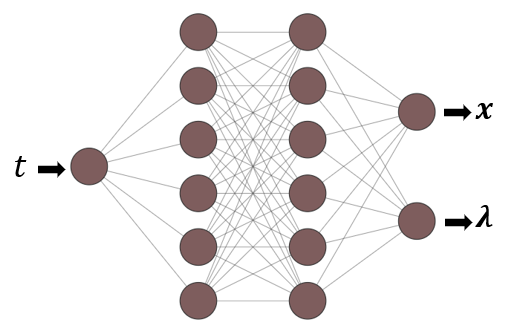
\includegraphics[width=0.55\linewidth,height=\textheight,keepaspectratio]{Chapter3_imgs/c22.PNG}

}

\caption{\label{fig-ch3-pinn-scalar}PINN architecture used for the
scalar and LTS problems}

\end{figure}%

\paragraph{Baseline Tanh Result}\label{baseline-tanh-result}

Using a Tanh activation function, a fully connected feedforward network
with two hidden layers of 16 neurons each yields the following
trainable-parameter budget:

\begin{longtable}[]{@{}
  >{\raggedright\arraybackslash}p{(\linewidth - 6\tabcolsep) * \real{0.1296}}
  >{\centering\arraybackslash}p{(\linewidth - 6\tabcolsep) * \real{0.2778}}
  >{\centering\arraybackslash}p{(\linewidth - 6\tabcolsep) * \real{0.2593}}
  >{\centering\arraybackslash}p{(\linewidth - 6\tabcolsep) * \real{0.3333}}@{}}
\caption{Trainable Parameters per Layer
(Tanh)}\label{tbl-ch3-trainable-tanh}\tabularnewline
\toprule\noalign{}
\begin{minipage}[b]{\linewidth}\raggedright
Layer
\end{minipage} & \begin{minipage}[b]{\linewidth}\centering
No of Weights
\end{minipage} & \begin{minipage}[b]{\linewidth}\centering
No of Biases
\end{minipage} & \begin{minipage}[b]{\linewidth}\centering
Total Parameters
\end{minipage} \\
\midrule\noalign{}
\endfirsthead
\toprule\noalign{}
\begin{minipage}[b]{\linewidth}\raggedright
Layer
\end{minipage} & \begin{minipage}[b]{\linewidth}\centering
No of Weights
\end{minipage} & \begin{minipage}[b]{\linewidth}\centering
No of Biases
\end{minipage} & \begin{minipage}[b]{\linewidth}\centering
Total Parameters
\end{minipage} \\
\midrule\noalign{}
\endhead
\bottomrule\noalign{}
\endlastfoot
Input to \(1^{st}\) Hidden Layer & \(1 \times 16 = 16\) & \(16\) &
\(16 + 16 = 32\) \\
\(1^{st}\) Hidden to \(2^{nd}\) Hidden Layer & \(16 \times 16 = 256\) &
\(16\) & \(256 + 16 = 272\) \\
\(2^{nd}\) Hidden to Output Layer & \(16 \times 2 = 32\) & \(2\) &
\(32 + 2 = 34\) \\
\textbf{Total} & \(16 + 256 + 32 = 304\) & \(16 + 16 + 2 = 34\) &
\(32 + 272 + 34 = 338\) \\
\end{longtable}

With this configuration, the training process converged to a total loss
of \(\mathcal{L} = 1.038 \times 10^{-4}\). When compared against the
analytical solution, the Root Mean Square (RMS) errors for the state and
costate variables are \(2.44 \times 10^{-3}\) and
\(3.64 \times 10^{-3}\), respectively. These results establish a
Tanh-based baseline that will be used as a reference in the subsequent
activation-function comparison.

\subsubsection{Linear Tangent Steering
Problem}\label{linear-tangent-steering-problem}

The LTS problem was introduced in Section~\ref{sec-ch2-lts} as a
classical time-optimal benchmark whose analytical solution is known. The
corresponding indirect optimality conditions were derived in Chapter 2
and yield the coupled state--costate system that the PINN must satisfy.

\paragraph{Indirect Formulation}\label{indirect-formulation}

The objective of the LTS problem is to minimize the final time \(t_f\).
The performance index is therefore

\begin{equation}\protect\phantomsection\label{eq-ch3-lts-objective}{
J = \int_{0}^{t_f} 1 \, dt = t_f.
}\end{equation}

According to Pontryagin's Maximum Principle, the Hamiltonian
\(\mathcal{H}\) is

\begin{equation}\protect\phantomsection\label{eq-ch3-lts-hamiltonian}{
\mathcal{H} = 1 + \lambda_1 \dot{x}_1 + \lambda_2 \dot{x}_2 + \lambda_3 \dot{x}_3 + \lambda_4 \dot{x}_4.
}\end{equation}

Substituting the expressions for the state derivatives,

\begin{equation}\protect\phantomsection\label{eq-ch3-lts-hamiltonian-sub}{
\begin{aligned}
\mathcal{H} &= 1 + \lambda_1 x_3 + \lambda_2 x_4 + \lambda_3 a \cos(u) + \lambda_4 a \sin(u).
\end{aligned}
}\end{equation}

The costate dynamics are obtained from

\begin{equation}\protect\phantomsection\label{eq-ch3-lts-costate-general}{
\dot{\lambda}_i = -\frac{\partial \mathcal{H}}{\partial x_i}, \quad i = 1,2,3,4.
}\end{equation}

which, for the LTS dynamics, evaluates to

\begin{equation}\protect\phantomsection\label{eq-ch3-lts-costate}{
\begin{aligned}
\dot{\lambda}_1 &= -\frac{\partial \mathcal{H}}{\partial x_1} = 0, \\
\dot{\lambda}_2 &= -\frac{\partial \mathcal{H}}{\partial x_2} = 0, \\
\dot{\lambda}_3 &= -\frac{\partial \mathcal{H}}{\partial x_3} = -\lambda_1, \\
\dot{\lambda}_4 &= -\frac{\partial \mathcal{H}}{\partial x_4} = -\lambda_2.
\end{aligned}
}\end{equation}

The optimal control minimizes the Hamiltonian with respect to \(u\):

\begin{equation}\protect\phantomsection\label{eq-ch3-lts-optimal-control}{
u^*(t) = \arg\min_u \mathcal{H} = \arg\min_u \left( \lambda_3 a \cos(u) + \lambda_4 a \sin(u) \right).
}\end{equation}

This can be rewritten as

\begin{equation}\protect\phantomsection\label{eq-ch3-lts-hu}{
\mathcal{H}_{u} = a \left( \lambda_3 \cos(u) + \lambda_4 \sin(u) \right),
}\end{equation}

and yields the closed-form optimal control

\begin{equation}\protect\phantomsection\label{eq-ch3-lts-u-optimal}{
u^*(t) = \tan^{-1}\left( \frac{\lambda_4(t)}{\lambda_3(t)} \right).
}\end{equation}

The boundary conditions for the LTS problem are:

\begin{itemize}
\tightlist
\item
  \textbf{Initial (fixed) conditions:}
\end{itemize}

\begin{equation}\protect\phantomsection\label{eq-ch3-lts-ic}{
x_1(0) = 0, \quad x_2(0) = 0, \quad x_3(0) = 0, \quad x_4(0) = 0
}\end{equation}

\begin{itemize}
\tightlist
\item
  \textbf{Final (partially fixed) conditions:}
\end{itemize}

\begin{equation}\protect\phantomsection\label{eq-ch3-lts-fc}{
x_2(t_f) = 5, \quad x_3(t_f) = 45, \quad x_4(t_f) = 0
}\end{equation}

\begin{itemize}
\tightlist
\item
  \textbf{Transversality condition (due to free final state):}
\end{itemize}

\begin{equation}\protect\phantomsection\label{eq-ch3-lts-transversality}{
\lambda_1(t_f) = 0 \quad \text{(since } x_1(t_f) \text{ is free)}
}\end{equation}

\paragraph{PINN Loss for the LTS
Problem}\label{pinn-loss-for-the-lts-problem}

In the PINN framework, the domain loss based on the residuals of the
state and costate ODEs is

\begin{equation}\protect\phantomsection\label{eq-ch3-lts-domain-loss}{
\mathcal{L}_{\text{residual}} = \frac{1}{N}\sum_{i=1}^{N} \left[ 
\sum_{j=1}^{4} \left( \frac{d x_j}{d t}(t_i) - f_j(\mathbf{x}(t_i), u(t_i)) \right)^2 
+ \sum_{j=1}^{4} \left( \frac{d \lambda_j}{d t}(t_i) - g_j(\boldsymbol{\lambda}(t_i)) \right)^2 
\right],
}\end{equation}

where \(f_j\) and \(g_j\) denote the right-hand sides of the state and
costate ODEs. The boundary loss enforces the known initial and final
values, including the transversality condition:

\begin{equation}\protect\phantomsection\label{eq-ch3-lts-bc-loss}{
\begin{aligned}
\mathcal{L}_{\text{BC}} = &\frac{1}{4} {\left( x_j(0) - x_{j,0} \right)^2 
+ \left( x_2(t_f) - 5 \right)^2 
+ \left( x_3(t_f) - 45 \right)^2 
+ \left( x_4(t_f) - 0 \right)^2 
+ \left( \lambda_1(t_f) \right)^2}
\end{aligned}
}\end{equation}

The complete loss function is therefore

\begin{equation}\protect\phantomsection\label{eq-ch3-lts-total-loss}{
\mathcal{L}_{\text{PINN}} = w_1 \mathcal{L}_{\text{residual}} + w_2 \mathcal{L}_{\text{BC}},
}\end{equation}

where \(w_1 + w_2 = 1\) are hyperparameters controlling the balance
between enforcing dynamics and boundary constraints. To place greater
emphasis on the control within the physics-informed loss, the
stationarity condition

\begin{equation}\protect\phantomsection\label{eq-ch3-lts-control-loss}{
\frac{\partial H}{\partial U} = 0 = -\lambda_3 \sin U + \lambda_4 \cos U
}\end{equation}

is also included as part of the loss formulation.

\paragraph{Hyperparameters and
Training}\label{hyperparameters-and-training}

For hyperparameter tuning, the training process employs a total of
\(30{,}000\) iterations, with a total loss threshold of \(10^{-4}\) used
as the primary stopping criterion. To enhance stability, a patience
mechanism \citep{sanchez2018real} is incorporated: once the loss falls
below \(10^{-4}\), training continues for an additional \(20\)
iterations to ensure the loss consistently remains under the specified
threshold.

The training procedure adopts a two-stage Optimization strategy. During
the first stage, \(90\%\) of the total iterations are executed using the
\textbf{Adam} optimizer with a learning rate of \(10^{-3}\), allowing
for efficient convergence in the initial phase. In the second stage, the
remaining \(10\%\) of iterations utilize the \textbf{L-BFGS} optimizer
for fine-tuning. The L-BFGS method is configured with a maximum of
\(50{,}000\) iterations, a history size of \(50\), and a strong Wolfe
line search condition.

This hybrid approach leverages the fast convergence properties of
first-order methods during early training, while exploiting the higher
accuracy of second-order methods in refining the solution as the loss
approaches its minimum.

As the analytical solution is available, the error of the control is
considered for tuning the network parameters. The diagram below shows
how the error varied for the Tanh activation function for different
number of hidden layers and nodes. The model with 3 hidden layers each
with 60 nodes (Figure~\ref{fig-ch3-hp-control}) shows the best results
and is used for the subsequent activation-function comparison.

\begin{figure}

\centering{

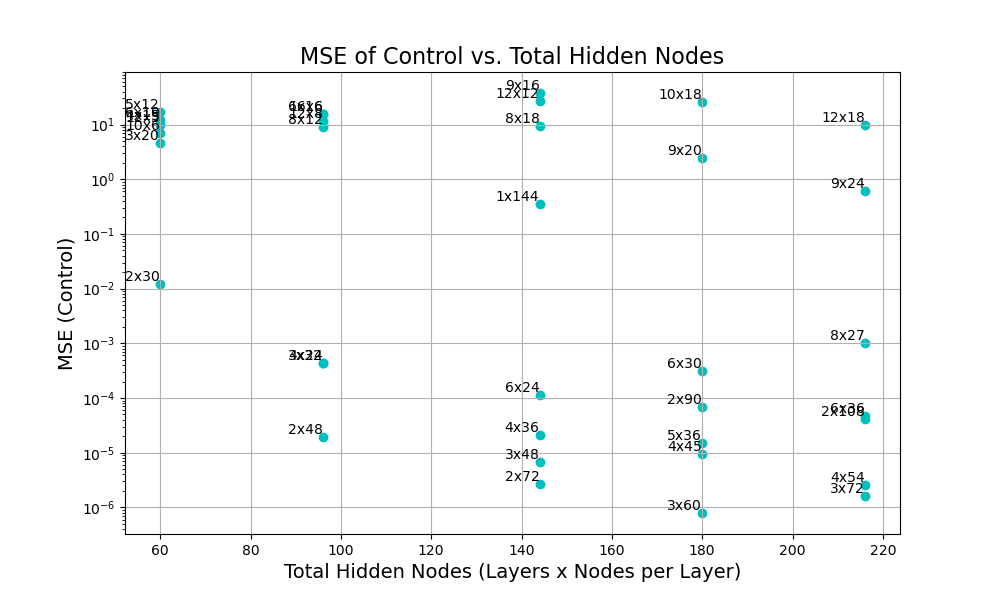
\includegraphics[width=0.75\linewidth,height=\textheight,keepaspectratio]{Chapter3_imgs/HP_control_diff_total_nodes.png}

}

\caption{\label{fig-ch3-hp-control}MSE error of Control for different
nodes and layers}

\end{figure}%

\begin{longtable}[]{@{}lr@{}}
\caption{Mean Squared Error (MSE) for States, Control, and Final
Time}\label{tbl-ch3-mse-lts}\tabularnewline
\toprule\noalign{}
Variable & MSE \\
\midrule\noalign{}
\endfirsthead
\toprule\noalign{}
Variable & MSE \\
\midrule\noalign{}
\endhead
\bottomrule\noalign{}
\endlastfoot
\(x_1\) & \(3.01 \times 10^{-9}\) \\
\(x_2\) & \(4.44 \times 10^{-9}\) \\
\(x_3\) & \(5.52 \times 10^{-8}\) \\
\(x_4\) & \(6.72 \times 10^{-8}\) \\
Control \(u\) & \(2.34 \times 10^{-5}\) \\
Error final Time \(\varepsilon_{t_f}\) & \(1.89 \times 10^{-6}\) \\
\end{longtable}

In the LTS case, careful tuning enabled the network to achieve mean
squared errors (MSE) as low as \(10^{-5}\) for the control. This level
of accuracy demonstrates the model's ability to learn the underlying
physics while maintaining smooth and stable control profiles.

\subsubsection{Effect of Activation Function on Model
Performance}\label{effect-of-activation-function-on-model-performance}

To investigate the role of activation functions in learning-based
control tasks, three variants are evaluated on the LTS problem: the
standard Tanh, Layer-wise Locally Adaptive Activation Functions (L-LAAF)
\citep{jagtap2022deep}, and Rowdy Adaptive Activation Functions (RAAF)
\citep{jagtap2022deep, ccelik2024optimal}. RAAF extends the modified
Tanh

\begin{equation}\protect\phantomsection\label{eq-ch3-modified-tanh}{
\sigma(x; \alpha) = \frac{e^{\alpha x} - e^{-\alpha x}}{e^{\alpha x} + e^{-\alpha x}},
}\end{equation}

where \(\alpha\) is a trainable parameter that scales the input, by
combining it with trigonometric terms:

\begin{equation}\protect\phantomsection\label{eq-ch3-raaf}{
\sigma_{\text{rowdy}}(x) = \sigma_{\text{base}}(x; \alpha) + \sum_{k=1}^N \beta_k \sin(k \omega x),
}\end{equation}

where \(\sigma_{\text{base}}(x; \alpha)\) is the adaptive Tanh, and
\(\beta_k\), \(\omega\) are trainable parameters controlling the
amplitude and frequency of the oscillations.

A key methodological point when comparing activation functions is that
RAAF introduces additional trainable parameters inside the activation
itself. For each neuron in the hidden layers,

\begin{equation}\protect\phantomsection\label{eq-ch3-raaf-extra}{
\text{Parameters}_\text{rowdy} = n_\text{hidden} \times \text{RAAF parameters},
}\end{equation}

so that the \emph{total} number of trainable parameters depends on the
activation-function choice, not just on the layer widths and depths.
Consequently, a comparison in which Tanh and RAAF share an
\emph{identical} network architecture will, in general, give RAAF a
strictly larger parameter budget and therefore an unfair advantage. A
fair comparison requires matching the \emph{total} trainable-parameter
count across activations by adjusting the number of hidden layers and/or
neurons accordingly. The results reported below for the LTS problem use
architectures that were tuned independently for each activation; an
explicitly equal-trainable-parameter comparison was not available in the
current results and is left as a TODO item for future work.

\paragraph{Accuracy Comparison (Mean Squared
Error)}\label{accuracy-comparison-mean-squared-error}

The Mean Squared Error (MSE) for key variables --- state components
\(x_1, x_2, x_3, x_4\), control input \(u\), and final time \(t_f\) ---
is computed post-training. The results are summarized below:

\begin{longtable}[]{@{}
  >{\raggedright\arraybackslash}p{(\linewidth - 6\tabcolsep) * \real{0.3333}}
  >{\raggedleft\arraybackslash}p{(\linewidth - 6\tabcolsep) * \real{0.2000}}
  >{\raggedleft\arraybackslash}p{(\linewidth - 6\tabcolsep) * \real{0.2667}}
  >{\raggedleft\arraybackslash}p{(\linewidth - 6\tabcolsep) * \real{0.2000}}@{}}
\caption{Comparison of MSE for different activation
functions}\label{tbl-ch3-mse-activation}\tabularnewline
\toprule\noalign{}
\begin{minipage}[b]{\linewidth}\raggedright
Variable
\end{minipage} & \begin{minipage}[b]{\linewidth}\raggedleft
RAAF
\end{minipage} & \begin{minipage}[b]{\linewidth}\raggedleft
L-LAAF
\end{minipage} & \begin{minipage}[b]{\linewidth}\raggedleft
Tanh
\end{minipage} \\
\midrule\noalign{}
\endfirsthead
\toprule\noalign{}
\begin{minipage}[b]{\linewidth}\raggedright
Variable
\end{minipage} & \begin{minipage}[b]{\linewidth}\raggedleft
RAAF
\end{minipage} & \begin{minipage}[b]{\linewidth}\raggedleft
L-LAAF
\end{minipage} & \begin{minipage}[b]{\linewidth}\raggedleft
Tanh
\end{minipage} \\
\midrule\noalign{}
\endhead
\bottomrule\noalign{}
\endlastfoot
\(x_1\) & \(2.10 \times 10^{-9}\) & \(1.74 \times 10^{-8}\) &
\(3.01 \times 10^{-9}\) \\
\(x_2\) & \(3.98 \times 10^{-9}\) & \(3.56 \times 10^{-9}\) &
\(4.44 \times 10^{-9}\) \\
\(x_3\) & \(7.03 \times 10^{-9}\) & \(9.57 \times 10^{-8}\) &
\(5.52 \times 10^{-8}\) \\
\(x_4\) & \(7.61 \times 10^{-9}\) & \(6.07 \times 10^{-8}\) &
\(6.72 \times 10^{-8}\) \\
Control \(u\) & \(2.01 \times 10^{-6}\) & \(1.69 \times 10^{-5}\) &
\(2.34 \times 10^{-5}\) \\
Final Time \(t_f\) & \(8.56 \times 10^{-7}\) & \(8.06 \times 10^{-7}\) &
\(1.89 \times 10^{-6}\) \\
\end{longtable}

RAAF yields the lowest MSE across most variables, especially in control
and states \(x_1\) and \(x_2\), indicating strong learning and
generalization. L-LAAF performs well, particularly in final time
\(t_f\), but exhibits higher errors in control and velocity states
(\(x_3\), \(x_4\)). Tanh shows the highest error in control and final
time, suggesting less adaptability to dynamic conditions.

The RAAF result for the scalar trajectory optimization problem also
supports this picture: on the scalar problem, RAAF achieves a total loss
of \(\mathcal{L} = 4.19 \times 10^{-5}\) and RMS errors of
\(6.54 \times 10^{-5}\) (state) and \(5.84 \times 10^{-5}\) (costate),
substantially lower than the Tanh baseline
(\(\mathcal{L} = 1.038 \times 10^{-4}\), RMS \(2.44 \times 10^{-3}\) and
\(3.64 \times 10^{-3}\)). The relevant RAAF trainable-parameter budget
for the scalar problem is

\begin{longtable}[]{@{}
  >{\raggedright\arraybackslash}p{(\linewidth - 8\tabcolsep) * \real{0.1111}}
  >{\centering\arraybackslash}p{(\linewidth - 8\tabcolsep) * \real{0.2083}}
  >{\centering\arraybackslash}p{(\linewidth - 8\tabcolsep) * \real{0.1944}}
  >{\centering\arraybackslash}p{(\linewidth - 8\tabcolsep) * \real{0.2361}}
  >{\centering\arraybackslash}p{(\linewidth - 8\tabcolsep) * \real{0.2500}}@{}}
\caption{Trainable Parameters per Layer
(RAAF)}\label{tbl-ch3-trainable-raaf}\tabularnewline
\toprule\noalign{}
\begin{minipage}[b]{\linewidth}\raggedright
Layers
\end{minipage} & \begin{minipage}[b]{\linewidth}\centering
No of Weights
\end{minipage} & \begin{minipage}[b]{\linewidth}\centering
No of Biases
\end{minipage} & \begin{minipage}[b]{\linewidth}\centering
RAAF Parameters
\end{minipage} & \begin{minipage}[b]{\linewidth}\centering
Total Parameters
\end{minipage} \\
\midrule\noalign{}
\endfirsthead
\toprule\noalign{}
\begin{minipage}[b]{\linewidth}\raggedright
Layers
\end{minipage} & \begin{minipage}[b]{\linewidth}\centering
No of Weights
\end{minipage} & \begin{minipage}[b]{\linewidth}\centering
No of Biases
\end{minipage} & \begin{minipage}[b]{\linewidth}\centering
RAAF Parameters
\end{minipage} & \begin{minipage}[b]{\linewidth}\centering
Total Parameters
\end{minipage} \\
\midrule\noalign{}
\endhead
\bottomrule\noalign{}
\endlastfoot
I/P to Hidden Layer & \(1 \times 20 = 20\) & \(20\) &
\(20 \times 3 = 60\) & \(20 + 20 + 60 = 100\) \\
Hidden to O/P Layer & \(20 \times 2 = 40\) & \(2\) & \(0\) &
\(40 + 2 + 0 = 42\) \\
\textbf{Total} & \(60\) & \(22\) & \(60\) & \(142\) \\
\end{longtable}

giving a total of \(142\) trainable parameters for RAAF against \(338\)
for the Tanh baseline on the scalar problem.

The qualitative picture of the PINN solution is illustrated in
Figure~\ref{fig-ch3-raaf-solution} and the comparison of total errors is
shown in Figure~\ref{fig-ch3-error-comparison}.

\begin{figure}

\centering{

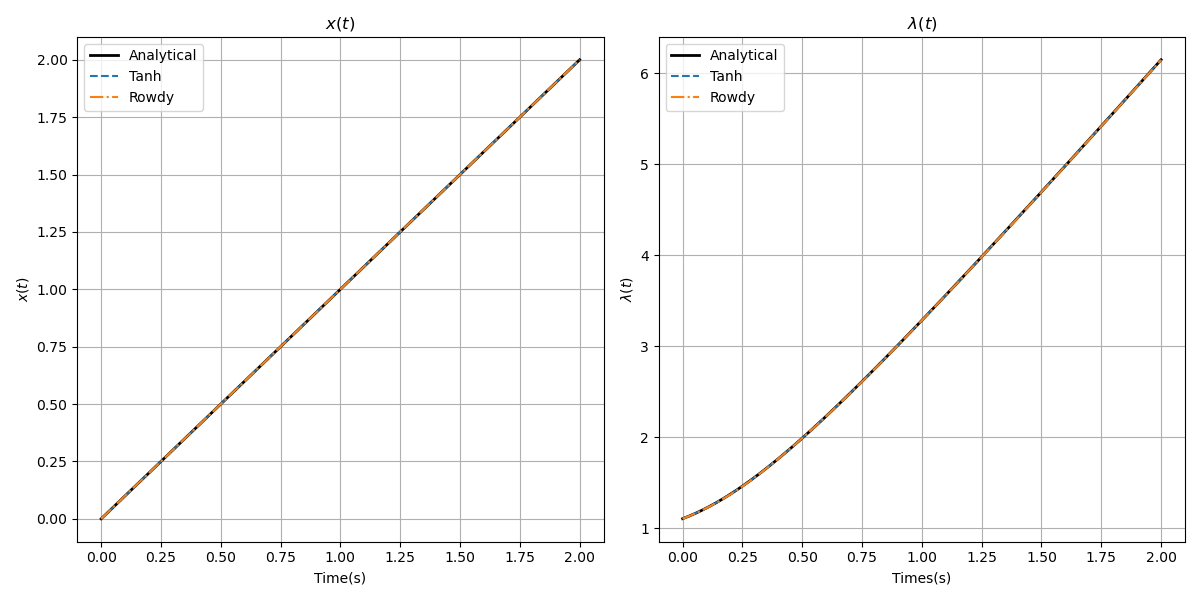
\includegraphics[width=0.75\linewidth,height=\textheight,keepaspectratio]{Chapter3_imgs/comp_tah_rowdy.png}

}

\caption{\label{fig-ch3-raaf-solution}PINNs Solution using RAAF}

\end{figure}%

\begin{figure}

\begin{minipage}[t]{0.50\linewidth}

\centering{

\pandocbounded{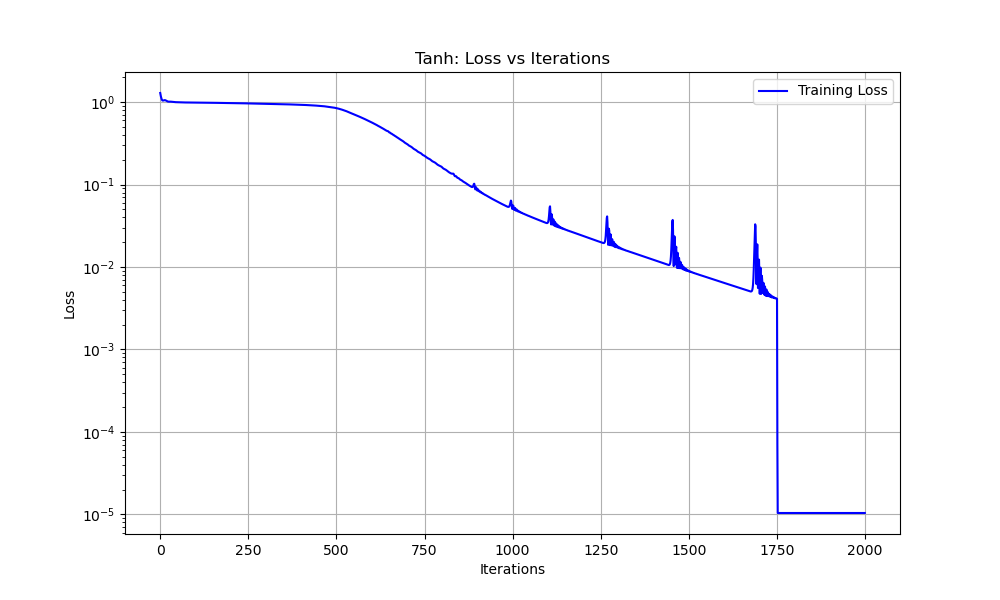
\includegraphics[keepaspectratio]{Chapter3_imgs/tanh_error.png}}

}

\subcaption{\label{fig-ch3-tanh-error}Total Error: Tanh.}

\end{minipage}%
%
\begin{minipage}[t]{0.50\linewidth}

\centering{

\pandocbounded{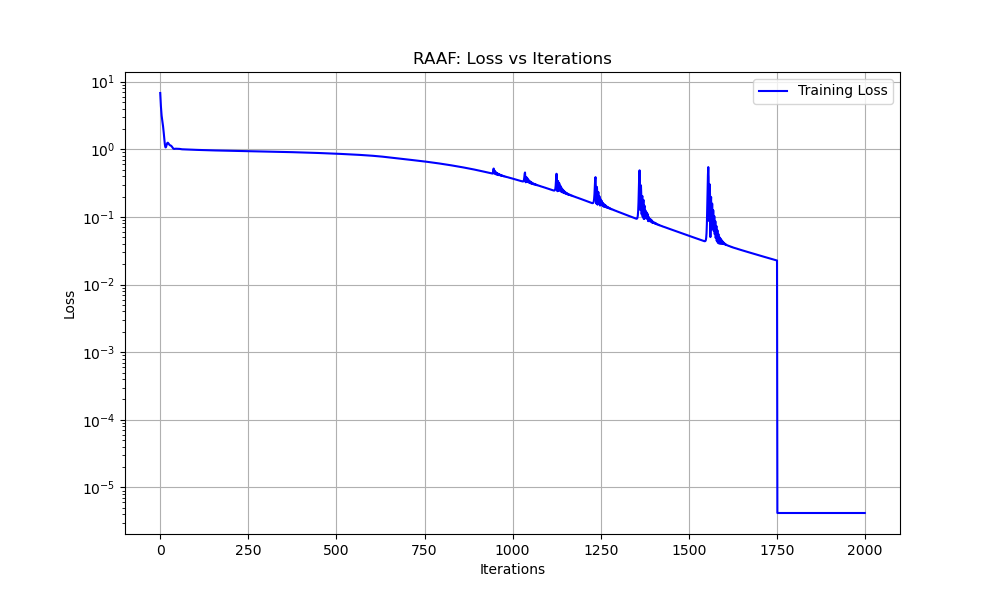
\includegraphics[keepaspectratio]{Chapter3_imgs/RAAF_error.png}}

}

\subcaption{\label{fig-ch3-raaf-error}Total Error: RAAF.}

\end{minipage}%

\caption{\label{fig-ch3-error-comparison}Comparison of the Total
errors.}

\end{figure}%

\paragraph{Computational Cost}\label{computational-cost}

The number of function evaluations and the total training time required
for each activation are summarized below:

\begin{longtable}[]{@{}lrrr@{}}
\caption{Comparison of Function Evaluations and Training
Time}\label{tbl-ch3-fe-time}\tabularnewline
\toprule\noalign{}
Metric & Tanh & L-LAAF & RAAF \\
\midrule\noalign{}
\endfirsthead
\toprule\noalign{}
Metric & Tanh & L-LAAF & RAAF \\
\midrule\noalign{}
\endhead
\bottomrule\noalign{}
\endlastfoot
Function Evaluations & 56625 & 56354 & 57871 \\
Training Time (s) & 782.23 & 1062.65 & 4637.72 \\
\end{longtable}

Tanh and L-LAAF are computationally cheaper, requiring fewer function
evaluations and less training time. RAAF takes significantly longer to
train, reflecting the additional complexity of its adaptive mechanism.
The relative computational expense can be expressed as the ratio of
training time against the Tanh baseline:

\[
\text{Training-Time Ratio}
=
\frac{T_{\text{activation}}}{T_{\text{Tanh}}}.
\]

Applied to the absolute numbers above, RAAF incurs a training-time ratio
of approximately \(5.93\times\) over Tanh (\(4637.72/782.23\)), while
L-LAAF incurs a ratio of approximately \(1.36\times\)
(\(1062.65/782.23\)). Despite its higher computational cost, RAAF
delivers superior accuracy, indicating a clear trade-off between
computational expense and learning performance. The choice of activation
function thus plays a crucial role in determining both learning accuracy
and computational efficiency: while RAAF achieves the best accuracy, it
comes at greater cost, whereas L-LAAF offers a balanced trade-off and
Tanh serves as a baseline with minimal computational demand. The
absolute wall-clock times reported above are hardware-dependent and
should therefore be interpreted through the relative ratios above rather
than as standalone figures.

\subsection{Parameterized PINN Solutions for
ODEs}\label{parameterized-pinn-solutions-for-odes}

In many engineering applications, the goal is not to solve a single
trajectory optimization problem but to generate solutions for an entire
\emph{class} of problems that differ only in their parameters. In the
LTS setting, for example, the terminal condition \(x_2(t_f)\) may vary
over a range, the initial state may be perturbed, or constants appearing
in the dynamics may take different values. Each such parameter choice
defines a separate two-point boundary value problem whose accuracy
depends strongly on the initial guess supplied to the nonlinear
optimizer. PINNs offer a natural way to amortize this cost: once a
network has been trained for one parameter value, its weights encode
information about the solution structure that can be reused to
initialize the next instance.

\subsubsection{Problem Parameterization}\label{problem-parameterization}

A trajectory optimization problem is parameterized when one or more of
its defining quantities is allowed to vary. Typical examples include the
initial state \(\mathbf{x}_0\), the terminal state \(\mathbf{x}(t_f)\),
the constants appearing in the governing dynamics, or auxiliary
quantities such as the time horizon. In the TPBVP formulation of an
indirect method, each such parameterization changes both the boundary
conditions and, through the costate transversality conditions, the shape
of the optimal trajectory. In the PINN setting, this corresponds to
retraining the network on a different set of residual and boundary
losses. Solving each instance independently is computationally
prohibitive when thousands of trajectories are required; the techniques
developed in the remainder of this section aim to reduce that cost by
transferring information across instances.

\subsubsection{Weight Initialization and
Interpolation}\label{weight-initialization-and-interpolation}

The key observation underlying all the techniques in this section is
that, when problem parameters change only slightly between instances,
the optimal network weights of one instance provide a useful starting
point for the next. After successfully training the network for a base
case (e.g., with \(x_2(t_f) = 5.0\) in the LTS problem), the trained
weights are saved. They capture meaningful features of the underlying
dynamics corresponding to that boundary condition, and can be reused ---
directly or after a simple extrapolation --- to initialize the network
for a slightly perturbed instance. This reuse significantly reduces the
number of iterations required for convergence: the network adapts
quickly to the new scenario since the dynamics remain similar, and the
pre-trained weights already encode a near-optimal structure of the
solution.

This idea generalizes the random-walk strategy used in earlier work on
the LTS problem \citep{izzo2017survey}: for a range of perturbations in
\(x_2(t_f)\), a linear interpolation of weights from nearby trained
cases was used to generate initial guesses, and these interpolated
weights provided good initialization even in untrained regions of the
parameter space, again accelerating convergence and improving training
stability. Instead of solving each variation from scratch, which is
computationally intensive, the PINNs leverage prior knowledge through
this weight-transfer strategy. This greatly enhances training efficiency
and enables real-time adaptability in solving trajectory optimization
problems such as the LTS, as illustrated in
Figure~\ref{fig-ch3-interpolation}.

\begin{figure}

\centering{

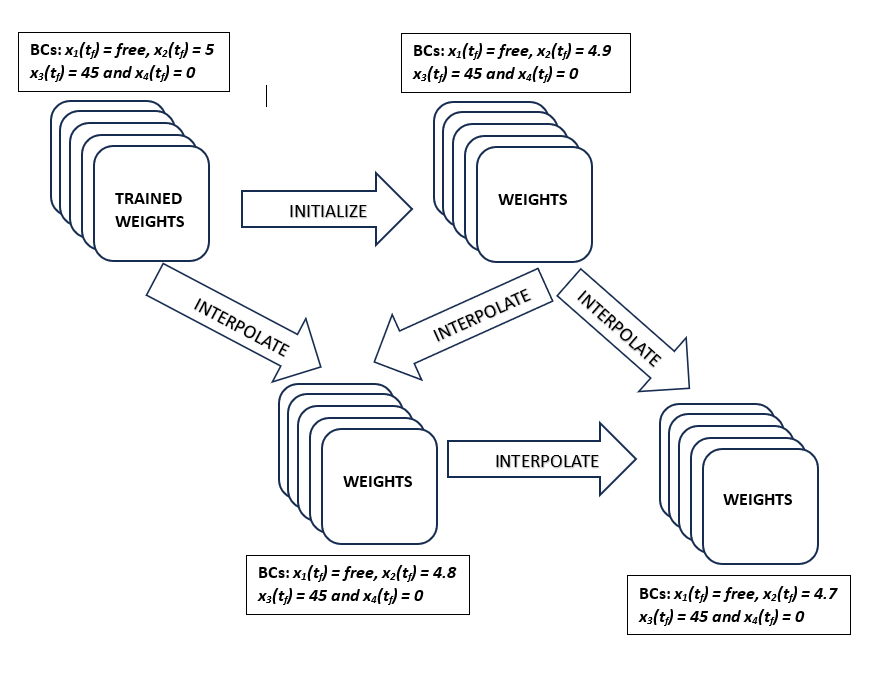
\includegraphics[width=0.75\linewidth,height=\textheight,keepaspectratio]{Chapter3_imgs/inter_process.PNG}

}

\caption{\label{fig-ch3-interpolation}Weight Initialization and
Interpolation}

\end{figure}%

\paragraph{Three Initialization
Strategies}\label{three-initialization-strategies}

For a parameterized problem in which the parameter \(x\) changes by
\(\Delta x\) from one instance to the next, three initialization
strategies are explicitly distinguished.

\textbf{Case 1 --- No warm start.} The new instance is solved without
using the previous instance's weights: the network is initialized from
random weights and trained to convergence. This is the most expensive
option, since no information is transferred across instances.

\textbf{Case 2 --- Izzo zeroth-order extrapolation.} The approach
followed by Izzo et al.~assumes that the weights at the new parameter
value are approximately equal to the weights at the previous parameter
value:

\[
W(x+\Delta x) \approx W(x).
\]

This is a \emph{zeroth-order} extrapolation: it transfers only the
function value, without any derivative information. It typically yields
a useful but coarse initialization.

\textbf{Case 3 --- Proposed first-order extrapolation.} The thesis
proposes a \emph{first-order} extrapolation that additionally uses the
local sensitivity of the weights with respect to the parameter:

\[
W(x+\Delta x)
\approx
W(x)
+
\Delta x
\frac{\partial W}{\partial x}.
\]

This first-order approximation captures the leading-order change in the
optimal weights when the parameter changes, and is expected to provide a
closer initialization than the zeroth-order alternative. The required
sensitivity \(\partial W / \partial x\) is obtained from the trained
network and the corresponding parameter perturbation; its exact form
follows the implementation in the thesis code.

\textbf{TODO --- quantitative comparison.} A side-by-side numerical
comparison of the three strategies (no warm start vs.~Izzo zeroth-order
vs.~proposed first-order) in terms of training iterations, function
evaluations, and wall-clock time is \emph{not yet available} in the
current results and is reserved here as a TODO item. The expected
quantitative summary, to be filled in once the corresponding experiments
are run, takes the form

\[
\text{Speedup}
=
\frac{T_{\text{baseline}}}{T_{\text{method}}},
\qquad
\text{Time Saving}
=
\frac{T_{\text{baseline}}-T_{\text{method}}}{T_{\text{baseline}}}\times 100\%,
\]

where \(T_{\text{baseline}}\) is the training time without warm starting
and \(T_{\text{method}}\) is the corresponding time under either the
zeroth-order or first-order strategy. Reporting relative savings, rather
than absolute wall-clock times, makes the comparison largely
hardware-independent, which is important because the absolute timings
depend on the underlying machine.

\paragraph{Recursive Weight Interpolation
Procedure}\label{recursive-weight-interpolation-procedure}

The interpolation approach used in this work is based on perturbing the
final state condition \(x_2(t_f)\) and exploiting the learned weights to
extrapolate weights for further perturbations.

The first perturbation is applied with \(\Delta x_2(t_f) = -0.1\), i.e.,
\(x_2(t_f) = 4.9\). The network for this modified final state is
initialized using the base weights (corresponding to \(x_2(t_f) = 5.0\))
and trained with the same stopping criterion as the base model. The loss
drops below \(10^{-4}\) within approximately 300 iterations, indicating
that the base weights significantly accelerated convergence. The network
successfully adapted to the new final state with a much smaller error
compared to training from scratch.

Once the network is trained for the perturbed final state
\(x_2(t_f) = 4.9\), the interpolation process is extended recursively to
generate weights for additional perturbations. The core idea is to use a
linear interpolation formula to predict new weights:

\begin{equation}\protect\phantomsection\label{eq-ch3-interpolation}{
w_{\text{new}} = m \cdot x_{2\text{(tf,new)}} + b,
}\end{equation}

where

\begin{equation}\protect\phantomsection\label{eq-ch3-interpolation-slope}{
m = \frac{w_2 - w_1}{x_{2\text{(tf,2)}} - x_{2\text{(tf,1)}}}, \quad b = w_1 - m \cdot x_{2\text{(tf,1)}}.
}\end{equation}

The weights corresponding to \(x_2(t_f) = 5.0\) and \(x_2(t_f) = 4.9\)
are used to extrapolate the weights for \(x_2(t_f) = 4.8\). After
verifying the performance of the network at \(x_2(t_f) = 4.8\), the
weights for \(x_2(t_f) = 4.9\) and \(4.8\) are used to extrapolate for
\(x_2(t_f) = 4.7\), and so on. This recursive interpolation continues by
always using the most recent two trained or extrapolated weight sets,
i.e.,

\begin{equation}\protect\phantomsection\label{eq-ch3-recursive}{
\text{Use } (w_{x_2 = 4.8}, w_{x_2 = 4.7}) \rightarrow w_{x_2 = 4.6}, \quad \text{and so on,}
}\end{equation}

until the final state condition \(x_2(t_f) = 4.0\) is reached. A similar
process is carried out in the forward direction. After training the
network at \(x_2(t_f) = 5.1\), the weights corresponding to
\(x_2(t_f) = 5.0\) and \(5.1\) are used to extrapolate for
\(x_2(t_f) = 5.2\), and this forward recursive interpolation is repeated
until \(x_2(t_f) = 6.0\) is reached. At each step, the accuracy of the
interpolated weights is evaluated by comparing them with weights
obtained through direct training for the corresponding final state
condition.

\begin{figure}

\begin{minipage}[t]{0.50\linewidth}

\centering{

\pandocbounded{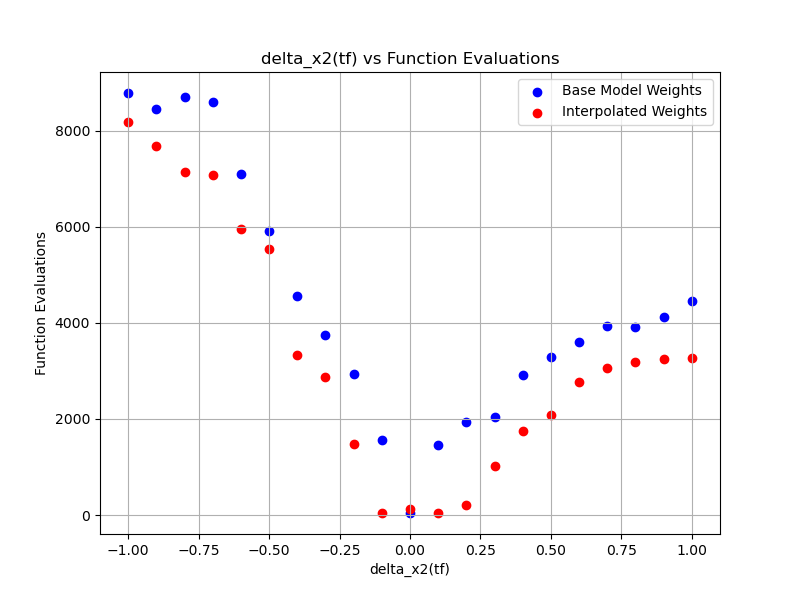
\includegraphics[keepaspectratio]{Chapter3_imgs/ppt_FE_intre.png}}

}

\subcaption{\label{fig-ch3-fe-eval}Number of Function Evaluations.}

\end{minipage}%
%
\begin{minipage}[t]{0.50\linewidth}

\centering{

\pandocbounded{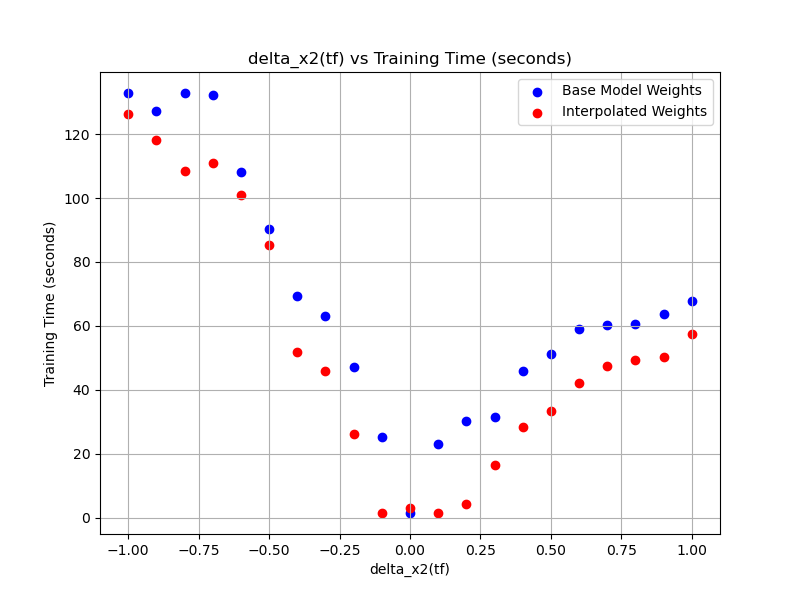
\includegraphics[keepaspectratio]{Chapter3_imgs/ppt_time_intre.png}}

}

\subcaption{\label{fig-ch3-train-time}Time for Training.}

\end{minipage}%

\end{figure}%

The recursive weight-interpolation procedure just described is a
specific instance of the zeroth-order transfer strategy of
Figure~\ref{fig-ch3-interpolation-results}. It illustrates, on a single
parameter (\(x_2(t_f)\)), how the same trained network can be repurposed
across many nearby instances at low cost.

Even with this warm-starting strategy, however, the estimated
computational cost of generating the full training dataset required by
downstream applications remains substantial. This motivates the
physics-informed simplification discussed next, in which the known
functional form of the optimal control is built directly into the
network.

\subsection{Simplified LTS Model with Trainable
Parameters}\label{simplified-lts-model-with-trainable-parameters}

In the original trajectory optimization framework using LTS, the control
input \(u\) is computed indirectly from the costate variables through
Pontryagin's Maximum Principle:

\begin{equation}\protect\phantomsection\label{eq-ch3-original-control}{
u(t) = \tan^{-1}\left(\frac{\lambda_4(t)}{\lambda_3(t)}\right)
}\end{equation}

This requires the neural network to output not only the state variables
\(x(t), y(t), u(t), v(t)\) but also the costate variables
\(\lambda_1(t), \lambda_2(t), \lambda_3(t), \lambda_4(t)\), resulting in
a total of eight outputs.

The simplified formulation avoids predicting costate variables
altogether. Leveraging the analytical structure of the LTS problem, the
optimal control \(u(t)\) is known to follow the form

\begin{equation}\protect\phantomsection\label{eq-ch3-simplified-control}{
u(t) = \tan^{-1} \left( \frac{c_1}{c_2} + \frac{c_3}{c_2} t \right),
}\end{equation}

where \(c_1, c_2, c_3\) are problem-dependent constants. In the
simplified model, these constants are treated as \emph{trainable
parameters} of the network, so that the network only needs to output the
four state variables. The control input \(u(t)\) is then computed using
the parameterized control law in
Equation~\ref{eq-ch3-simplified-control}, bypassing the need to estimate
costates. The constants \(c_1, c_2, c_3\) are learned alongside the
network weights during training. During forward passes, \(u(t)\) is
computed directly from the equation using the current value of time
\(t\) and the learned parameters.

This physics-informed choice has three concrete consequences that the
experiments quantify. First, by eliminating the need to predict
costates, the network output size is halved --- from eight outputs to
four --- which reduces the required network size. Second, the resulting
smaller network requires less computational training time. Third, as a
result of the first two effects, the simplified model remains accurate
on the states while drastically reducing the control error, as shown in
the comparison below.

\begin{longtable}[]{@{}lrr@{}}
\caption{Error comparison between original RAAF and Simplified LTS: RAAF
model.}\label{tbl-ch3-simplified}\tabularnewline
\toprule\noalign{}
Metric & RAAF & Simplified LTS: RAAF \\
\midrule\noalign{}
\endfirsthead
\toprule\noalign{}
Metric & RAAF & Simplified LTS: RAAF \\
\midrule\noalign{}
\endhead
\bottomrule\noalign{}
\endlastfoot
State 1 Error & \(2.1008 \times 10^{-9}\) & \(4.3835 \times 10^{-9}\) \\
State 2 Error & \(3.9782 \times 10^{-9}\) & \(4.5787 \times 10^{-9}\) \\
State 3 Error & \(7.0327 \times 10^{-9}\) & \(5.0759 \times 10^{-9}\) \\
State 4 Error & \(7.6105 \times 10^{-9}\) & \(7.8337 \times 10^{-9}\) \\
Control Error & \(2.0105 \times 10^{-6}\) & \(3.2782 \times 10^{-8}\) \\
Error in \(t_f\) & \(8.5635 \times 10^{-7}\) &
\(1.5023 \times 10^{-7}\) \\
\end{longtable}

The simplified LTS model maintains low state errors while significantly
reducing the control error. To compare the training-time savings in a
hardware-independent manner, the absolute times are converted into a
ratio against the original RAAF model:

\[
\text{Training-Time Ratio}
=
\frac{T_{\text{simplified}}}{T_{\text{original}}}
=
\frac{2276.0}{4637.72}
\approx
0.491,
\]

which corresponds to a time saving of approximately \(50.9\%\).
Additionally, the number of function evaluations is reduced to \(57477\)
(against \(57871\) for the original RAAF), further confirming the
efficiency of the proposed approach. This trade-off between model
simplicity and performance reduces network complexity and improves
computational efficiency without compromising accuracy, and exemplifies
how hybridizing physics-based insight with learning-based models can
yield both performance and interpretability benefits.

\subsection{Limitations}\label{limitations}

As the number of states increases in an optimal control problem --- for
instance, from four to five by including an additional state such as the
pitch angle and its corresponding ODE --- the total loss during PINN
training has been observed to diverge. This divergence is largely due to
the added complexity introduced by the additional differential
constraints, which significantly increases the number of residual terms
the network must learn to satisfy. Each new state variable contributes
both a state ODE and its associated costate equation in the Hamiltonian
formalism, effectively doubling the number of ODE constraints.
Consequently, the loss function becomes composed of many competing
objectives --- state dynamics, costate dynamics, and boundary/initial
conditions --- that can conflict during optimization.

This issue has been identified in the literature as a major limitation
in PINN-based methods for optimal control. Mowlavi and Nabi
\citep{mowlavi2022} highlighted that in PDE-constrained optimal control
problems, the presence of multiple differential constraints ---
especially when each comes with a state and costate component --- can
destabilize training due to the imbalance in the loss function.
Similarly, Barry-Straume et al. \citep{barry2022controlpinns} observed
that as more equations are embedded into the PINN loss (e.g., due to
additional state variables), the learning dynamics degrade, resulting in
either stagnation or divergence of the total loss. New et al.
\citep{new2022} further showed empirically that increasing the number of
coupled ODEs, even in relatively simple settings, leads to poor
convergence behavior due to the ill-conditioning of the optimization
landscape and vanishing or exploding gradients.

\newpage

\section{Theory of Functional Connections (TFC) for Solving Optimal
Control
Problems}\label{theory-of-functional-connections-tfc-for-solving-optimal-control-problems}

To overcome the limitations of Physics-Informed Neural Networks (PINNs)
in solving optimal control problems (OCPs), this chapter introduces the
Theory of Functional Connections \citep{mortari2017least} (TFC), a
mathematically rigorous framework derived from the Theory of Connections
(ToC). While PINNs have been proposed as a mesh-free alternative for
solving the Two-Point Boundary Value Problems (TPBVPs) arising from
indirect formulations of OCPs, they often struggle with convergence when
the number of states and costates increases. The resulting complexity in
the loss function, composed of multiple ODE residuals, boundary
conditions, and transversality constraints, leads to gradient imbalance
and divergence during training, limiting the reliability of PINNs in
high-dimensional or tightly coupled systems.

TFC addresses these issues by embedding boundary and initial conditions
directly into the functional form of the solution using constrained
expressions. This eliminates the need for explicitly penalizing
constraint violations in the loss function, as is done in PINNs, and
transforms the problem into an unconstrained least-squares Optimization
over the free function components. As a result, TFC avoids the
instability and sensitivity associated with neural network-based solvers
while maintaining high accuracy and computational efficiency.

This chapter explores the application of TFC to optimal control problems
\citep{furfaro2020least}, with case studies including energy-optimal
planetary landing and space interception problems. Through detailed
simulations and comparisons, it is demonstrated that TFC provides a
robust and scalable alternative to both traditional numerical solvers
and PINN-based approaches, particularly in scenarios where
neural-network solutions tend to diverge.

\subsection{Solution to TPBVPs Using the
TFC}\label{solution-to-tpbvps-using-the-tfc}

This section describes the methodology for solving nonlinear Two-Point
Boundary Value Problems (TPBVPs) using the Theory of Functional
Connections (TFC). The approach transforms the original
boundary-constrained differential problem into an unconstrained problem
by embedding the boundary conditions analytically into the solution
structure.

\subsubsection{General Formulation of the
TVBVP}\label{general-formulation-of-the-tvbvp}

We consider the linear boundary value problem \citep{furfaro2020least}:

\[
\dot{x}(t) + 2t\,x(t) = \sin(t), \quad t \in [0, 1], \quad x(0) = 0,\quad x(1) = 1.
\]

To embed the boundary conditions, we define a constrained expression
using the Theory of Functional Connections:

\[
x(t) = g(t) + (1 - t)x(0) + t x(1) - (1 - t) g(0) - t g(1).
\]

Substituting the known boundary values \(x(0) = 0\), \(x(1) = 1\), this
simplifies to:

\[
x(t) = g(t) + t - (1 - t)g(0) - t g(1).
\]

Differentiating this expression gives:

\[
\dot{x}(t) = \dot{g}(t) + 1 - g(1) + g(0).
\]

Substituting \(x(t)\) and \(\dot{x}(t)\) into the original differential
equation:

\[
\dot{g}(t) + 1 - g(1) + g(0) + 2t\left( g(t) + t - (1 - t)g(0) - t g(1) \right) = \sin(t).
\]

Expanding the right-hand side:

\[
\dot{g}(t) + 2t g(t) + g(0)(1 - 2t + 2t^2) + g(1)(-1 - 2t^2) + (1 + 2t^2) = \sin(t).
\]

Rewriting, we define the residual function:

\[
R(t) = \dot{g}(t) + 2t g(t) + \gamma_0(t) g(0) + \gamma_1(t) g(1) + r(t) - \sin(t),
\]

where:

\[
\gamma_0(t) = 1 - 2t + 2t^2, \quad \gamma_1(t) = -1 - 2t^2, \quad r(t) = 1 + 2t^2.
\]

We now express the free function \(g(t)\) as a linear combination of
basis functions:

\[
g(t) = \sum_{i=1}^{m} c_i \phi_i(t), \quad \dot{g}(t) = \sum_{i=1}^{m} c_i \dot{\phi}_i(t).
\]

At a set of collocation points \(\{ t_j \}_{j=1}^N \in [0,1]\), we
evaluate the residual:

\[
R(t_j) = \sum_{i=1}^{m} c_i \left[ \dot{\phi}_i(t_j) + 2t_j \phi_i(t_j) - \gamma_0(t_j)\phi_i(0) - \gamma_1(t_j)\phi_i(1) \right] + r(t_j) - \sin(t_j).
\]

This defines a linear least-squares system \(A\mathbf{c} = \mathbf{b}\),
where:

\[
A_{ji} = \dot{\phi}_i(t_j) + 2t_j \phi_i(t_j) - \gamma_0(t_j)\phi_i(0) - \gamma_1(t_j)\phi_i(1),
\quad
b_j = \sin(t_j) - r(t_j).
\]

Solving this system yields the coefficients \(\{ c_i \}\), from which we
reconstruct:

\[
g(t) = \sum_{i=1}^{m} c_i \phi_i(t),
\quad
g(0) = \sum_{i=1}^{m} c_i \phi_i(0),
\quad
g(1) = \sum_{i=1}^{m} c_i \phi_i(1).
\]

The final solution is then:

\[
x(t) = g(t) + t - (1 - t)g(0) - t g(1).
\]

This function \(x(t)\) satisfies the original boundary conditions
exactly and approximates the solution to the differential equation by
minimizing the residual in a least-squares sense.

\subsubsection{Energy Optimal Planetary Landing via Theory of
Connections}\label{energy-optimal-planetary-landing-via-theory-of-connections}

In this section, we consider the energy-optimal landing problem of a
spacecraft descending towards a planetary surface. The simplified
dynamics of the spacecraft assume constant gravitational acceleration
\(\mathbf{g}\) and control input in the form of thrust-induced
acceleration \(\mathbf{a}_C(t)\). The equations of motion governing the
system are given by:

\[
\dot{\mathbf{r}}(t) = \mathbf{v}(t),
\]

\[
\dot{\mathbf{v}}(t) = \mathbf{g} + \mathbf{a}_C(t),
\]

where \(\mathbf{r}(t) \in \mathbb{R}^3\) is the position vector and
\(\mathbf{v}(t) \in \mathbb{R}^3\) is the velocity vector of the
spacecraft.

The objective is to minimize the total control effort, which corresponds
to minimizing the energy expenditure. This is represented by the
performance index:

\begin{equation}\protect\phantomsection\label{eq-ch4-j}{
J = \frac{1}{2} \int_{t_0}^{t_f} \|\mathbf{a}_C(t)\|^2 \, dt.
}\end{equation}

The boundary conditions specify the initial and final states:

\[
\mathbf{r}(t_0) = \mathbf{r}_0, \quad \mathbf{v}(t_0) = \mathbf{v}_0,
\]

\[
\mathbf{r}(t_f) = \mathbf{r}_f = \mathbf{0}, \quad \mathbf{v}(t_f) = \mathbf{v}_f = \mathbf{0}.
\]

To solve this optimal control problem, we apply Pontryagin's Minimum
Principle (PMP). The Hamiltonian is defined as:

\begin{equation}\protect\phantomsection\label{eq-ch4-hamiltonian}{
\mathcal{H} = \frac{1}{2} \|\mathbf{a}_C\|^2 + \boldsymbol{\lambda}_r^T \mathbf{v} + \boldsymbol{\lambda}_v^T (\mathbf{g} + \mathbf{a}_C),
}\end{equation}

where \(\boldsymbol{\lambda}_r\) and \(\boldsymbol{\lambda}_v\) are the
costate vectors associated with \(\mathbf{r}(t)\) and \(\mathbf{v}(t)\),
respectively.

From the optimality condition
\(\partial \mathcal{H}/\partial \mathbf{a}_C = 0\), we obtain the
optimal control law:

\begin{equation}\protect\phantomsection\label{eq-ch4-ac}{
\mathbf{a}_C = -\boldsymbol{\lambda}_v.
}\end{equation}

Substituting this into the state and costate equations yields the
two-point boundary value problem (TPBVP):

\[
\dot{\mathbf{r}} = \mathbf{v}, \quad \dot{\boldsymbol{\lambda}}_r = \mathbf{0},
\]

\[
\dot{\mathbf{v}} = \mathbf{g} - \boldsymbol{\lambda}_v, \quad \dot{\boldsymbol{\lambda}}_v = -\boldsymbol{\lambda}_r.
\]

An analytical solution for the acceleration profile that satisfies these
conditions is given by:

\[
\mathbf{a}_C(t) = \frac{6}{t_{go}^2} (\mathbf{r}_f - \mathbf{r}_0) - \frac{4}{t_{go}} (\mathbf{v}_f - \mathbf{v}_0) - \mathbf{g},
\]

where \(t_{go} = t_f - t\) is the time-to-go until touchdown.

To solve this problem using the Theory of Connections (ToC), we
construct constrained expressions for \(\mathbf{r}(t)\) and
\(\mathbf{v}(t)\) that automatically satisfy the boundary conditions.
These expressions take the form:

\[
\mathbf{r}(t) = \mathbf{g}_r(t) + \mathbf{r}_0 + (t - t_0) \left( \frac{\mathbf{r}_f - \mathbf{r}_0}{t_f - t_0} - \mathbf{g}_r(t_f) \right),
\]

\[
\mathbf{v}(t) = \mathbf{g}_v(t) + \mathbf{v}_0 + (t - t_0) \left( \frac{\mathbf{v}_f - \mathbf{v}_0}{t_f - t_0} - \mathbf{g}_v(t_f) \right),
\]

where \(\mathbf{g}_r(t)\) and \(\mathbf{g}_v(t)\) are free functions
expanded in a basis of Chebyshev polynomials:

\begin{equation}\protect\phantomsection\label{eq-ch4-chebyshev}{
\mathbf{g}_r(t) = \sum_{k=0}^{m} c_k T_k(\tau(t)), \quad \tau(t) \in [-1, 1],
}\end{equation}

with \(T_k\) denoting the Chebyshev polynomials of the first kind and
\(c_k\) the unknown coefficients.

The residuals of the transformed equations of motion are then minimized
in a least-squares sense by discretizing the time domain at \(N\)
collocation points and solving the resulting overdetermined linear
system:

\begin{equation}\protect\phantomsection\label{eq-ch4-lstsq}{
\boldsymbol{\xi} = (A^T A)^{-1} A^T \mathbf{b},
}\end{equation}

where \(A\) is the matrix formed from the basis functions and
\(\mathbf{b}\) is the vector of discretized residuals.

For simulation, the initial position and velocity are given by
\(\mathbf{r}_0 = [160, 0, 1500]^T\) m and
\(\mathbf{v}_0 = [100, 0, -75]^T\) m/s. The final conditions are zero
position and velocity, and gravitational acceleration is assumed
constant as \(\mathbf{g} = [0, 0, -1.625]^T\) m/s\(^2\). The total
flight time is taken as \(t_f = 50\) s.

\begin{figure}

\centering{

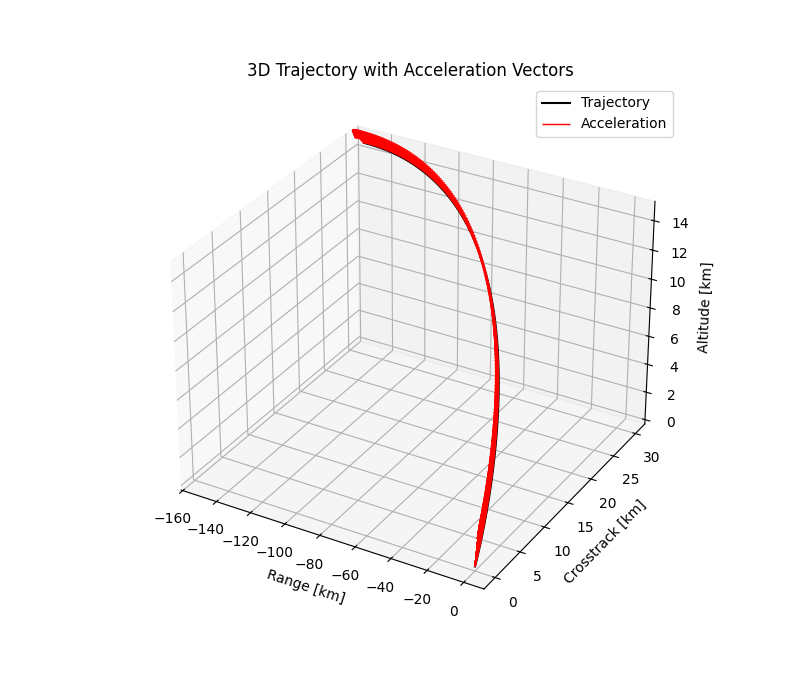
\includegraphics[width=0.75\linewidth,height=\textheight,keepaspectratio]{Chapter4_imgs/3d_trajectory.png}

}

\caption{\label{fig-ch4-3d-trajectory}Trajectory.}

\end{figure}%

The ToC-based solver produces accurate estimates of the state and
costate trajectories, and the resulting control input minimizes the
energy cost functional. The numerical solution agrees well with results
obtained via standard MATLAB solvers such as \texttt{bvp4c} and with
analytical predictions, demonstrating both the effectiveness and
computational efficiency of the ToC approach in solving energy-optimal
planetary landing problems.

\newpage

\section*{Conclusion and Future work}\label{conclusion-and-future-work}
\addcontentsline{toc}{section}{Conclusion and Future work}

\subsection*{Conclusion}\label{conclusion}
\addcontentsline{toc}{subsection}{Conclusion}

This work explored various approaches to solving trajectory Optimization
problems, a fundamental challenge in aerospace engineering. Beginning
with an overview of the trajectory Optimization landscape, the thesis
introduced the foundational concepts, including objective functions,
constraints, and classifications such as direct and indirect methods. It
highlighted the trade-offs between robustness, accuracy, and
computational complexity inherent to each approach.

The second part delved into classical direct methods such as the
Trapezoidal and Hermite-Simpson discretizations. These methods transform
the continuous-time optimal control problem into a nonlinear programming
problem by discretizing state and control trajectories. While the
Hermite-Simpson method demonstrated improved accuracy over the
Trapezoidal method, both faced limitations in handling discontinuous
control profiles, such as chattering in bang-bang problems. To address
these, regularization techniques and optimizer refinements were applied,
which significantly improved the smoothness and accuracy of the control
profiles.

The indirect method was then introduced, which formulates the trajectory
Optimization problem using the Pontryagin Maximum Principle. By
converting the optimal control problem into a two-point boundary value
problem (TPBVP), the method yields high-accuracy solutions. However,
solving the resulting coupled state-costate equations proved to be
highly sensitive to initial guesses and numerically unstable, especially
for problems involving complex or stiff dynamics.

To overcome these challenges, the study implemented Physics-Informed
Neural Networks (PINNs) as an alternative solver for the coupled ODEs.
PINNs offered a mesh-free, data-free solution by embedding the physical
constraints into the network's loss function. The effectiveness of the
PINN was tested on scalar and vector optimal control problems, and its
accuracy was enhanced using custom activation functions like the Rowdy
Adaptive Activation Function (RAAF). While PINNs showed promise,
especially with well-tuned architectures and initializations, their
performance was sensitive to hyperparameters and required careful
training.

Finally, the Theory of Functional Connections (TFC) was presented as a
highly efficient and accurate method for solving trajectory Optimization
problems. By embedding the boundary conditions analytically into the
solution structure, TFC converts constrained differential equations into
unconstrained Optimization problems. The TFC-based least-squares method
demonstrated excellent accuracy, reduced computational complexity, and
exact satisfaction of boundary conditions. Unlike traditional
collocation or shooting methods, TFC eliminates the need for numerical
enforcement of constraints, making it highly suitable for solving both
linear and nonlinear TPBVPs.

\subsection*{Future Work}\label{future-work}
\addcontentsline{toc}{subsection}{Future Work}

As PINNs effectively solve coupled state and costate equations with
reasonable accuracy, their performance may degrade as the complexity of
the problem increases, particularly when the number of ODEs grows
significantly. To address this limitation, advanced architectures such
as Physics-Informed Deep Operator Networks (DeepONets) can be employed.
DeepONets are designed to learn operators, offering superior accuracy
and scalability compared to traditional PINNs for high-dimensional and
complex dynamical systems.

Once the state and costate trajectories are obtained through DeepONets,
the resulting data can be utilized to train a standard DNN. This DNN
would act as a mapping function from the initial state of the system to
the optimal control policy, providing a computationally efficient
framework for real-time control applications. Such a hybrid approach
leverages the strengths of operator-learning frameworks and traditional
neural networks, offering a promising avenue for solving challenging
trajectory Optimization problems.

In addition, future work can explore the integration of the Theory of
Functional Connections (TFC) with nonlinear control problems and
higher-dimensional systems. While the current application has been
limited to one-dimensional or low-order linear problems, extending TFC
to more general nonlinear time-varying systems could significantly
broaden its applicability. Investigating adaptive basis selection,
sparse representations, and GPU-accelerated implementations could
further enhance its computational performance. Moreover, combining TFC
with machine learning techniques to estimate parameters or control laws
from data, while preserving the analytical constraint embedding of TFC,
may lead to highly efficient hybrid solvers that retain interpretability
and accuracy.

\newpage


\bibliography{bibliography.bib}



\end{document}
